\documentclass[pdflatex,11pt]{../aghdoc_version2}
% \documentclass{../aghdoc}               % przy kompilacji programem latex
\usepackage[polish]{babel}
\usepackage[utf8]{inputenc}

% dodatkowe pakiety
\usepackage[hidelinks]{hyperref}
\usepackage{enumerate}
\usepackage{listings}
\usepackage{caption}
\usepackage{amsmath}
\usepackage{algorithm2e}
% TODO przenieść do aghdoc
\newcommand{\code}[1]{\texttt{#1}}

% żeby stopki były zastosowane do stron gdzie rozpoczyna się rozdział
\usepackage{etoolbox}
\patchcmd{\chapter}{\thispagestyle{plain}}{\thispagestyle{fancy}}{}{}

\lstloadlanguages{TeX}

\lstset{
  literate={ą}{{\k{a}}}1
           {ć}{{\'c}}1
           {ę}{{\k{e}}}1
           {ó}{{\'o}}1
           {ń}{{\'n}}1
           {ł}{{\l{}}}1
           {ś}{{\'s}}1
           {ź}{{\'z}}1
           {ż}{{\.z}}1
           {Ą}{{\k{A}}}1
           {Ć}{{\'C}}1
           {Ę}{{\k{E}}}1
           {Ó}{{\'O}}1
           {Ń}{{\'N}}1
           {Ł}{{\L{}}}1
           {Ś}{{\'S}}1
           {Ź}{{\'Z}}1
           {Ż}{{\.Z}}1
}

%---------------------------------------------------------------------------

\author{Tomasz Kasprzyk, Daniel Ogiela, Jakub Stępak}
\shortauthor{T. Kasprzyk, D. Ogiela, J.Stępak}

\titlePL{System obliczający wyniki wyborów dla uogólnienia systemu k-Borda}

\shorttitlePL{System obliczający wyniki wyborów dla uogólnienia systemu k-Borda} % skrócona wersja tytułu jeśli jest bardzo długi

\thesistypePL{Dokumentacja techniczna}

\supervisorPL{dr hab. inż. Piotr Faliszewski}

\date{2016}

\departmentPL{Katedra Informatyki}

\facultyPL{Wydział Informatyki, Elektroniki i Telekomunikacji}

\setlength{\cftsecnumwidth}{10mm}

% umożliwienie żeby domyślnie dokument nie robił wcięć poza wybranymi (\indent w tym miejscu)

\newlength\tindent
\setlength{\tindent}{\parindent}
\setlength{\parindent}{0pt}
\renewcommand{\indent}{\hspace*{\tindent}}

\fancypagestyle{plain}{%
\fancyhf{} % clear all header and footer fields
\fancyhead[R]{\bfseries \thepage}
\fancyfoot[C]{System obliczający wyniki wyborów dla uogólnienia systemu k-Borda} % except the center
\renewcommand{\headrulewidth}{0.5pt}
\renewcommand{\footrulewidth}{0.5pt}}

%---------------------------------------------------------------------------

\begin{document}

\titlepages

\tableofcontents\thispagestyle{fancy}


%----------------------------------------------------------------------------
\chapter{Dziedzina problemu}
\label{cha:dziedzina_problemu}

\section{Metoda obliczania wyników wyborów}
\label{sec:metoda_obliczania_wynikow_wyborow}

\subsection{Metoda Bordy}
\label{subsec:metoda_bordy}

Niech $v$ będzie głosem nad zbiorem kandydatów $C$. Wynik według Bordy kandydata $c$ w $v$ jest równy \begin{equation}
\beta(i)=||C||-i,
\end{equation}
gdzie $i$- pozycja kandydata w ciągu $v$.\\
Wynik $c$ w wyborach jest sumą wyników $c$ u każdego z wyborców


\subsection{Metoda k-Borda}
\label{subsec:metoda_k_borda}

Rozszerzenie metody Bordy. Wynik, zamiast dla jednego kandydata, obliczany jest dla ciągu kandydatów. $f_{kB}$- funkcja zadowolenia z komitetu, $(i_1,\dots, i_k)$- ciąg pozycji kandydatów
\begin{equation}
f_{kB}=\sum_{j=1}^{k} \beta(i_j)
\end{equation}

\paragraph{Przyklad}
$C=\{c_1,c_2,c_3,c_4\}$ - zbiór kandydatów,
$v=(c_2,c_1,c_4,c_3)$ - głos
Niech $k = 2$ (wybory $2$ spośród $4$)
$w=(c_4,c_3)$.
Najpierw określamy pozycje kandydatów z komitetu $w$ w $v$:
$pos_v(w)=(3,4)$, zatem wynik komitetu w dla głosu v wynosi
$f_{kB}(3,4) = (3) + (4) = ||C|| - 3 ) + ( ||C|| - 4 ) = 1 + 0 = 1$


\subsection{Uogólnienie - system $\ell_p$-Borda}
\label{subsec:system_ell_p_borda}

Zanim wprowadzone zostanie pojęcie uogólnionego systemu $k-Borda$ warto przypomnieć wzór na normę\,$\ell_p$
\subsubsection{Norma $\ell_p$}
\label{subsubsection:norma_ell_p}
\begin{equation}
\ell_p(x_1,x_2,\dots, x_n) = \sqrt[p]{x_1^p+x_2^p+\dots+x_n^p}
\end{equation}


Wówczas, w uogólnionej wersji metody $k-Borda$, funkcja zadowolenia $f_{kB}$ (1.2) zostaje uzależniona również od parametru $p$ ze wzoru (1.3). Norma liczona jest z wyników według Bordy, $\beta(i)$ (1.1).\\Wzór uogólniony funkcji zadowolenia przyjmuje zatem postać:
\begin{equation}
f_{\ell_pB}(p,(i_1,\dots,i_k))=\sqrt[p]{[(i_1)]^p+[(i_2)]^p+...+[(i_k)]^p}
\end{equation}

Systemy $k-Borda$ i \textit{Chamberlina-Couranta} są szczególnymi przypadkami zdefiniowanego powyżej systemu $\ell_p-Borda$:\\
Dla \, $p = 1$, \, $l_1$:
\begin{equation}
f_{\ell_pB}(1,(i_1, \dots ,i_k)) = \beta(i_1) + \beta(i_2) + \dots + \beta(ik) = f_{kB}(i_11, \dots,i_k)
\end{equation}
Dla \, $p= \infty$, \, $l_{\infty}={max}$:

\begin{multline}
\begin{split}
f_{\ell_pB}(\infty,(i_1, \dots ,i_k))\\
&=\lim\limits_{p \to \infty} \sqrt[p]{\beta\left[(i_1)\right]^p+\beta\left[(i_2)\right]^p+ \dots +\left[\beta(i_k)\right]^p}\\
&=\max{\beta(i_1),\beta(i_2),\dots,\beta(i_k)} = \beta(i_1)=f_{CC}
\end{split}
\end{multline}

\section{Format danych wejściowych}
\label{sec:format_danych_wejsciowych}
Struktura danych wejściowych została zaczerpnięta z zestawów danych zamieszczonych na stronie Pref\,Lib \footnote{\url{http://www.preflib.org/data/format.php\#soc}}. Wykorzystywanym typem zestawów danych są zestawy SOC \footnote{SOC - \textit{Strict Orders - Complete List}}
\footnote{Szczegółowe opisy wyborów odnoszących się do poszczególnych plików można znaleźć pod adresem\\\url{http://www.preflib.org/data/index.php\#ed}}.\\
Zgodnie ze specyfikacją, każdy prawidłowy plik z rozszerzeniem \textit{.soc} posiada profil będący całkowitą, przejściową i asymetryczną relacją na grupie obiektów.\\
\textit{Preferencje} definiowane są jako ciągi liter oddzielone przecinkami, przykładowo:\\
\code{A, B, C;}\\
Powyższy zapis oznacza, że, spośród trzech opcji A, B, C, A jest bardziej preferowana niż B i C oraz B jest bardziej preferowana niż C. Relacja silnego porządku jest wówczas określana przez przecinek.\\
\\
Format pliku \textit{.soc}:\\
\code{<liczba kandydatów> \\
1, <nazwa kandydata> \\
2, <nazwa kandydata> \\
… \\
<liczba kandydatów>, <nazwa kandydata> \\
<liczba głosujących>, <liczba głosów policzonych>, <liczba unikalnych głosów> \\
<liczba powtórzeń głosu>, <głos> \\
… \\
<liczba powtórzeń głosu>, <głos>}\\
\\
Przy czym \code{<głos>} to pojedyncza \textit{preferencja} opisana powyżej.

\chapter{Architektura Django}
\textit{Django} to framework webowy napisany w \textit{Pythonie}. Dostarcza wysokopoziomowych
abstrakcji pozwalających na szybkie i wygodne pisanie przejrzystych aplikacji. \\ \\
Jego architektura koncepcyjnie przypomina wzorzec architektoniczny \textit{Model-View-Controller},
jednak, jak przyznają sami twórcy
\footnote{\url{https://docs.djangoproject.com/en/1.10/faq/general/}{\\Django appears to be a MVC framework, but you call the Controller the “view”, and the View the “template”. How come you don’t use the standard names?}}
, \textit{Django} nie do końca wpasowuje się w klasyczne
ujęcie \textit{MVC}. \\ \\
\textit{Django} dostarcza mapowania obiekto-relacyjnego, dzięki którym całość modeli można ująć
w \textit{Pythonie}. Wygodny \textit{ORM} zazwyczaj wystarcza do obsługi bazy danych, jednak zawsze
istnieje możliwość użycia bezpośrednio \textit{SQL}. \\ \\
Widoki w \textit{Django} spełniają dwojaką funkcję - służą zarówno przekazaniu danych do
wyświetlenia, jak i ich modyfikacji. W wyświetleniu danych użytkownikowi pośredniczą
szablony (\textit{templates}), które \"opakowują\" przekazane dane do postaci \textit{HTML'a}, który może wyświetlić przeglądarka internetowa. Dzięki temu wybór danych, jakie mają zostać pokazane
użytkownikowi, jest oddzielony od samego sposobu ich prezentacji. \\ \\
Za kontroler z klasycznego \textit{MVC} można uznać sam framework dostarczający wspomnianej
obsługi bazy danych czy mapowania adresów \textit{URL} do poszczególnych widoków.

\chapter{Opis modułów}
\label{cha:opis_modulow}

\section{Moduł administracji kont}
\subsection{Opis ogólny}
Moduł odpowiedzialny za zarządzanie kontami użytkowników. Umożliwia czynności
logowania, wylogowania oraz rejestracji. Nie współpracuje z innymi modułami. Korzysta
jedynie z bazy danych w celu weryfikacji użytkowników.

\subsection{Komponenty programowe}
Komponenty programowe dla tego modułu znajdują się w pakiecie \code{ecs.accounts} \\ \\
{
\centering
\begin{tabular}{|c|c|c|}
\hline
\textbf{Typ komponentu} & \textbf{Komponenty} & \textbf{Wykorzystanie} \\
\hline
widoki & klasa \code{LoginView} & logowanie \\
\cline{2-3}
 & klasa \code{RegisterView} & rejestracja \\
\hline
szablony & \code{login.html} & logowanie \\
\cline{2-3}
 & \code{register.html} & rejestracja \\
\hline
formularze & klasa \code{LoginForm} & logowanie \\
\cline{2-3}
 & klasa \code{RegistrationForm} & rejestracja \\
\hline
\end{tabular}
}

\section{Moduł zarządzania wyborami}
\subsection{Opis ogólny}
Moduł odpowiedzialny za administrację wyborami i ich wynikami. Umożliwia podstawowe
operacje na wyborach i ich wynikach oraz nawigację między nimi. Pozwala na wyświetlenie
listy wszystkich wyborów i ich wyników, stworzenie nowych wyborów lub wyniku, czy
usunięcie wyborów. W celu wykonania niektórych zadań współpracuje z modułem obliczania
wyników wyborów oraz modułem wizualizacji wyborów i ich wyników. Jest to najbardziej
rozbudowany moduł.
\clearpage

\subsection{Komponenty programowe}
% \usepackage{array} is required
Komponenty programowe dla tego modułu znajdują się w pakietach:  \code{ecs.elections.views} (widoki), \code{ecs.elections.templates} (szablony) i \code{ecs.elections.forms} (formularze).\\ \\
\begin{tabular}{|c|c|p{6cm}|}
\hline
\textbf{Typ komponentu} & \textbf{Komponenty} & \textbf{Wykorzystanie} \\
\hline
widoki & klasa \code{ElectionListView} & wyświetlenie listy wszystkich wyborów \\
\cline{2-3}
 & klasa \code{ElectionCreateView} & stworzenie wyborów \\
\cline{2-3}
 & klasa \code{ElectionDeleteView} & usunięcie wyborów \\
\cline{2-3}
 & klasa \code{ElectionDetailView} & wyświetlenie informacji szczegółowych o
danych wyborach \\
\cline{2-3}
 & klasa \code{ResultCreateView} & stworzenie wyniku dla danych wyborów -
wyświetlenie formularza określającego
parametry wyniku \\
\cline{2-3}
 & klasa \code{ResultDetailsView} & wyświetlenie danego wyniku danych
wyborów \\
\cline{2-3}
 & klasa \code{ResultDeleteView} & usuwanie pojedynczego wyniku wyborów \\
\hline
szablony & \code{election\_list.html} & wyświetlenie listy wszystkich wyborów,
usunięcie wyborów - strona wyświetlana po pomyślnym usunięciu wyborów \\
\cline{2-3}
 & \code{election\_create.html} & stworzenie wyborów \\
\cline{2-3}
 & \code{election\_details.html} & stworzenie wyborów - strona
wyświetlana po pomyślnym stworzeniu wyborów,
wyświetlenie informacji szczegółowych o
danych wyborach \\
\cline{2-3}
 & \code{election\_delete.html} & usunięcie wyborów \\
\cline{2-3}
 & \code{result\_create.html} & stworzenie nowego wyniku wyborów -
strona z formularzem \\
\cline{2-3}
 & \code{result\_details.html} & wyświetlenie danego wyniku danych
wyborów \\
\cline{2-3}
 & \code{result\_delete.html} & potwierdzenie usunięcia rezultatu \\
\hline
formularze & klasa \code{ElectionForm} & stworzenie wyborów \\
\cline{2-3}
 & klasa \code{ResultForm} & stworzenie wyniku dla danych wyborów -
formularz określający parametry wyniku \\
\hline
\end{tabular}
\clearpage

\section{Moduł wizualizacji wyborów i wyników wyborów}
\subsection{Opis ogólny}
Moduł odpowiedzialny za stworzenie wykresu \textit{2D} wizualizującego wybory i jego wyniki.
Wizualizacja dotyczy tylko wyborów wygenerowanych z rozkładu normalnego.\\ Wyborcy i
kandydaci są reprezentowani jako punkty na płaszczyźnie. Punkty reprezentujące wyborców
i kandydatów mają na wykresie odmienne kolory. Na wykresie wyników wyborów punkty
reprezentujące zwycięzców wyborów są powiększone.\\ Moduł współpracuje z modułem
zarządzania wyborów, który zleca mu zadanie wizualizacji wyborów lub jego wyników. W
celu wykonania zadania moduł wizualizacji wyborów i wyników wyborów pobiera dane z
bazy danych.

\subsection{Komponenty programowe}
Komponenty programowe dla tego modułu znajdują się w pakietach:  \code{ecs.elections.views} oraz \code{ecs.utils.chart\_views} \\ \\
\begin{tabular}{|c|c|p{5cm}|}
\hline
\textbf{Typ komponentu} & \textbf{Komponenty} & \textbf{Wykorzystanie} \\
\hline
widoki & klasa \code{ChartMixin} & pobranie danych potrzebnych do
wygenerowania wykresów (punkty, tytuł
wykresu, serii danych), dziedziczy po
klasie \code{View} \\
\cline{2-3}
 & klasa \code{ElectionChartView} & wizualizacja wyborów, klasa dziedziczy
po klasie \code{ScatterChartMixin}, pobranie
współrzędnych kandydatów i wyborców \\
\cline{2-3}
 & klasa \code{ResultChartView} & wizualizacja wyników wyborów, klasa
dziedziczy po klasie \code{ScatterChartMixin},
pobranie współrzędnych kandydatów,
wyborców oraz zwycięzców \\
\cline{2-3}
& klasa \code{AlgorithmsChartView} & zestawia dla danych wyborów czasy wykonania obliczeń  przez rózne algorytmy dla róznych wartości parametru $p$\\
\hline

\end{tabular}
\clearpage

\section{Moduł generacji i wczytywania wyborów}
\subsection{Opis ogólny}
Moduł odpowiedzialny za generację wyborów z rozkładu normalnego oraz wczytywanie
wyborów z pliku formatu \textit{.soc}. Moduł współpracuje z modułem zarządzania wyborami,
któremu zleca po wykonaniu swoich zadań, stworzenie i wysłanie użytkownikowi
odpowiedniej strony internetowej. Moduł zapewnia wygenerowanie wyborów z rozkładu normalnego według wskazanych parametrów oraz walidację danych przy wczytywaniu
wyborów z pliku. Po stworzeniu wyborów moduł komunikuje się z bazą danych w celu
utrwalenia wyborów.

\subsection{Komponenty programowe}
Komponenty programowe dla tego modułu znajdują się w pakietach:  \code{ecs.elections.views} (widoki), \code{ecs.elections.templates} (szablony) oraz \code{ecs.elections.forms} (formularze).\\ \\
\begin{tabular}{|c|c|p{5cm}|}
\hline
\textbf{Typ komponentu} & \textbf{Komponenty} & \textbf{Wykorzystanie} \\
\hline
Widoki & klasa \code{ElectionLoadDataFormView} & wczytanie wyborów z pliku \\
\cline{2-3}
 & klasa
\code{ElectionGenerateDataFormView} & generacja wyborów z rozkładu
normalnego \\
\hline
Szablony & \code{election\_load\_data.html} & strona z formularzem do
wskazania pliku \\
\cline{2-3}
 & \code{election\_generate\_data.html} & strona z formularzem do
wskazania parametrów wyborów i
rozkładu normalnego \\
\cline{2-3}
 & \code{election\_details.html} & strona wyświetlana po
poprawnym wczytaniu danych z
pliku \\
\hline
Formularze & klasa \code{ElectionLoadDataForm} & wczytanie z pliku \\
\hline
\end{tabular}

\section{Moduł obliczania wyników wyborów}
\subsection{Opis ogólny}
Moduł odpowiedzialny za obliczanie wyników wyborów. Zapewnia różne algorytmy do
wykonania zadania. Użytkownik ma wybór między algorytmem genetycznym, dwoma
algorytmami zachłannymi oraz algorytmem typu brute-force. Moduł współpracuje z modułem
zarządzania wyborami, który zleca mu wykonanie zadania.
\subsection{Komponenty programowe}
Wszystkie komponenty programowe dotyczące modułu obliczania wyników wyborów
zawierają się w pakiecie \code{ecs.elections.algorithms}. \\
Klasy odpowiedzialne za poszczególne algorytmy:
\begin{itemize}
\item \code{BruteForce} - odpowiedzialna za algorytm typu brute-force
\item \code{GreedyAlgorithm} - odpowiedzialna za algorytm zachłanny zależny od parametru $p$
\item \code{GreedyCC} - odpowiedzialna za algorytm zachłanny niezależny od parametru $p$
\item \code{GeneticAlgorithm} - odpowiedzialna za algorytm genetyczny
\end{itemize}

\section{Moduł URL Resolver}
\subsection{Opis ogólny}
Moduł odpowiedzialny za przekazywanie żądań otrzymywanych przez klienta do
odpowiednich modułów.

\subsection{Komponenty programowe}
Przyporządkowania żądań użytkownika do odpowiednich modułów (adresów URL do
widoków) znajdują się w pakiecie \code{ecs.elections.urls}.

\chapter{Współpraca modułów i innych komponentów}
\section{Diagram komunikacji}
\begin{center}
\centerline{\includegraphics[scale=0.65]{pics/Diagram_Komunikacji.png}}
\captionof{figure}{Diagram komunikacji}
\end{center}

\section{Ścieżki przejść}
\subsection{Logowanie}
\begin{enumerate}
\item Użytkownik za pomocą przeglądarki internetowej wysyła żądanie logowania.
\item Moduł URL Resolver kieruje żądanie do modułu administracji kont.
\clearpage
\item Moduł administracji kont przesyła do przeglądarki stronę z formularzem do
zalogowania (pole \textit{Username} i \textit{Password}).
\item Użytkownik wypełnia formularz i za pomocą przeglądarki internetowej wysyła
uzupełniony formularz.
\item Moduł URL Resolver przekazuje żądanie do modułu administracji kont.
\item Moduł administracji kont przeprowadza uwierzytelnienie użytkownika.
\item W zależności od rezultatu uwierzytelnienia podjęte są trzy możliwe akcje:
	\begin{itemize}
	\item jeżeli uwierzytelnienie powiodło się, Moduł administracji kont loguje użytkownika 		i wysyła do
	przeglądarki stronę z wiadomością o sukcesie logowania
	\item jeżeli podana nazwa użytkownika nie istnieje w bazie, Moduł administracji kont 			wysyła do
	przeglądarki internetowej stronę z formularzem do zalogowania (pole
	\textit{Username} i \textit{Password}) i z informacją o nieistnieniu podanej nazwy
	użytkownika. Następuje przejście do kroku nr $4$
	\item jeżeli podana nazwa użytkownika istnieje w bazie, ale podane hasło jest
nieprawidłowe, Moduł administracji kont wysyła do przeglądarki internetowej stronę z
formularzem do zalogowania (pole \textit{Username} i \textit{Password}) i z informacją o
błędnym haśle. Następuje przejście do kroku nr $4$
	\end{itemize}
\end{enumerate}

\subsection{Wylogowanie}
\begin{enumerate}
\item Użytkownik za pomocą przeglądarki internetowej wysyła żądanie wylogowania.
\item Moduł URL Resolver kieruje żądanie do modułu administracji kont.
\item Moduł administracji kont wylogowuje użytkownika i przesyła do przeglądarki stronę
domową aplikacji.
\end{enumerate}

\subsection{Rejestracja}
\begin{enumerate}
\item Użytkownik za pomocą przeglądarki internetowej wysyła żądanie zarejestrowania
użytkownika.
\item Moduł URL Resolver kieruje żądanie do modułu administracji kont.
\item Moduł administracji kont przesyła do przeglądarki stronę z formularzem do rejestracji
(pola \textit{E-mail}, \textit{Username}, \textit{Password}, \textit{First name} i \textit{Last name}).
\item Użytkownik wypełnia formularz i za pomocą przeglądarki internetowej wysyła
uzupełniony formularz.
\item Moduł URL Resolver przekazuje żądanie do modułu administracji kont.
\item Moduł administracji kont przeprowadza walidację danych.
\clearpage
\item W zależności od rezultatu walidacji:
	\begin{itemize}
	\item jeżeli się powiodła, Moduł administracji kont tworzy konto nowego użytkownika, 			zapisuje je do
	bazy danych, loguje użytkownika do nowo utworzonego konta i przesyła do
	przeglądarki stronę z wiadomością o sukcesie logowania
	\item w przeciwnym wypadku, zostaje wysłana do przeglądarki strona z
	formularzem do rejestracji wraz z informacją o znalezionym problemie.
	Następuje przejście do kroku nr $4$
	\end{itemize}
\end{enumerate}

\subsection{Wyświetlenie listy wszystkich wyborów}
\begin{enumerate}
\item Użytkownik klikając przycisk \textit{Your elections} na stronie, wysyła za pomocą
przeglądarki internetowej żądanie wyświetlenia listy swoich wyborów.
\item Moduł URL Resolver kieruje żądanie do modułu zarządzania wyborami (widok
\textit{ElectionListView}).
\item Moduł zarządzania wyborami kieruje zapytanie do bazy danych o obiekty
reprezentujące wybory danego użytkownika.
\item Po pobraniu z bazy potrzebnych danych moduł zarządzania wyborami za pomocą
szablonu\,\code{election\_list.html} tworzy stronę i wysyła do przeglądarki internetowej
użytkownika.
\end{enumerate}

\subsection{Stworzenie wyborów}
\begin{enumerate}
\item Użytkownik klikając przycisk \textit{New election} na stronie, wysyła za pomocą
przeglądarki internetowej żądanie stworzenie nowych wyborów.
\item Moduł URL Resolver kieruje żądanie do modułu zarządzania wyborami (widok
\textit{ElectionCreateView}).
\item Widok posiada zdefiniowany szablon \code{election\_create.html} i formularz \textit{ElectionForm}.
Wykorzystując te komponenty tworzy i wysyła do użytkownika stronę z formularzem.
\item Użytkownik wypełnia formularz (pola \textit{Name} i \textit{Commitee size}) i wysyła uzupełniony
formularz.
\item Moduł URL Resolver kieruje żądanie do modułu zarządzania wyborami (widok
\textit{ElectionCreateView}).
\item Widok wykorzystując klasę formularza pobiera dane z formularza, tworzy nowy
obiekt wyborów i zapisuje go do bazy.
\item Widok wykorzystując szablon \code{election\_details.html} tworzy stronę i wysyła ją do
przeglądarki użytkownika.
\end{enumerate}
\clearpage

\subsection{Usunięcie wyborów}
\begin{enumerate}
\item Użytkownik klikając ikonę kosza na stronie, wysyła za pomocą przeglądarki
internetowej żądanie usunięcia wyborów.
\item Moduł URL Resolver kieruje żądanie do modułu zarządzania wyborami (widok
\textit{ElectionDeleteView}).
\item Widok posiada zdefiniowany szablon \code{election\_delete.html}, który wykorzystuje do
stworzenia i wysłania strony potwierdzającej akcję użytkownika.
\item Użytkownik potwierdza chęć usunięcia wyborów przez naciśnięcie przycisku \textit{Yes,
delete this.} (W przypadku wyboru przycisku \textit{No, cancel} akcja nie zostaje przeprowadzona a użytkownik zostaje przeniesiony na stronę z listą swoich
wyborów).
\item Moduł URL Resolver kieruje żądanie do modułu zarządzania wyborami (widok
\textit{ElectionDeleteView}).
\item Widok usuwa wybory z bazy danych i wykorzystując szablon \code{election\_list.html} tworzy
i wysyła stronę do przeglądarki internetowej użytkownika.
\end{enumerate}

\subsection{Wyświetlenie informacji szczegółowych dla danych wyborów}
\begin{enumerate}
\item Użytkownik klikając na link wyborów na stronie z listą swoich wyborów, wysyła za
pomocą przeglądarki internetowej żądanie wyświetlenia informacji szczegółowych
dla danych wyborów.
\item Moduł URL Resolver kieruje żądanie do modułu zarządzania wyborami\,(widok\,\code{ElectionDetailView}).
\item Widok pobiera z bazy danych listę głosujących oraz listę wyników wyborów.
\item Jeżeli wybory zostały wygenerowane z rozkładu normalnego, widok przekierowuje
działanie programu do modułu wizualizacji wyborów i wyników wyborów (widok
\code{ElectionChartView}). Jeżeli wybory nie zostały wygenerowane z rozkładu normalnego, następuje przejście do kroku nr $6$
\item Widok pobiera z bazy danych obiekty będące punktami \textit{2D} reprezentującymi
wyborców i kandydatów. Ustawia parametry wykresu a następnie wysyła wszystkie
dane z powrotem do widoku \code{ElectionDetailView} umożliwiając stworzenie wykresu.
\item Widok wykorzystując szablon \code{election\_details.html} tworzy i wysyła stronę do
przeglądarki użytkownika.
\end{enumerate}
\clearpage

\subsection{Stworzenie nowego wyniku dla danych wyborów}
\begin{enumerate}
%do poprawki
\item Użytkownik klikając na link \textit{Add new result} na stronie ze szczegółowymi informacjami
o danych wyborach, wysyła za pomocą przeglądarki internetowej żądanie stworzenia
nowego wyniku dla danych wyborów.
\item Moduł URL Resolver kieruje żądanie do modułu zarządzania wyborami (widok
\textit{ResultCreateView}).
\item Widok wykorzystując formularz \textit{ResultForm} i szablon \code{result\_create.html} tworzy oraz
wysyła do użytkownika stronę z formularzem do określenia parametrów wyniku (pola:
parametr $p$ do obliczania normy oraz typ algorytmu).
\item Użytkownik wypełnia formularz i wysyła go do systemu.
\item Moduł URL Resolver kieruje żądanie do modułu zarządzania wyborami (widok
\code{ResultCreateView}).
\item Widok wczytuje dane z formularza, pobiera z bazy danych obiekt reprezentujący
wybory a następnie przekierowuje działanie programu do modułu obliczania wyników
wyborów przekazując konieczne parametry.
\item Moduł obliczania wyników wyborów liczy zwycięzców wyborów za pomocą
odpowiedniego algorytmu. Następnie przekazuje sterowanie z powrotem do widoku
\code{ResultCreateView} przekazując wyniki.
\item Widok zapisuje wynik do bazy danych i przechodzi do ścieżki \textit{Wyświetlenie
informacji szczegółowych dla danych wyborów}.
\end{enumerate}
\subsection{Wyświetlenie szczegółowych informacji o danym wyniku danych
wyborów}
\begin{enumerate}
\item Użytkownik klikając na link danego wyniku wyborów na stronie ze szczegółowymi
informacjami o danych wyborach, wysyła za pomocą przeglądarki internetowej
żądanie wyświetlenia szczegółowych informacji o danym wyniku dla danych
wyborów.
\item Moduł URL Resolver kieruje żądanie do modułu zarządzania wyborami (widok
\code{ResultDetailsView}).
\item Widok pobiera z bazy danych informacje o zwycięzcach danych wyborów.
\item Jeżeli wybory zostały wygenerowane z rozkładu normalnego, widok przekierowuje
działanie programu do modułu wizualizacji wyborów i wyników wyborów (widok
\code{ResultChartView}). Jeżeli wybory nie zostały wygenerowane z rozkładu normalnego, następuje przejście do kroku nr $6$.
\clearpage
\item Widok pobiera z bazy danych obiekty będące punktami \textit{2D} reprezentującymi
wyborców, kandydatów i zwycięzców. Ustawia parametry wykresu a następnie
wysyła wszystkie dane z powrotem do widoku \code{ResultDetailsView}, umożliwiając
stworzenie wykresu.
\item Widok wykorzystując szablon \code{result\_details.html} tworzy i wysyła stronę do
przeglądarki użytkownika.
\end{enumerate}

\subsection{Wczytanie wyborów z pliku .soc}
\begin{enumerate}
\item Użytkownik klikając na przycisk \textit{Load data from file} na stronie ze szczegółowymi
informacjami o danych wyborach, wysyła za pomocą przeglądarki internetowej
żądanie wczytania wyborów z pliku \textit{.soc}.
\item Moduł URL Resolver kieruje żądanie do modułu generacji i wczytywania wyborów (widok
\code{ElectionLoadDataFormView}).
\item Widok wykorzystując formularz \code{ElectionLoadDataForm} i szablon
\code{election\_load\_data.html} tworzy oraz wysyła do użytkownika stronę z formularzem do
wybrania pliku, z którego będą wczytywane wybory.
\item Użytkownik wskazuje plik i wysyła uzupełniony formularz do systemu.
\item Moduł URL Resolver kieruje żądanie do modułu generacji i wczytywania wyborów (widok
\code{ElectionLoadDataFormView}).
\item Widok parsuje plik wejściowy i waliduje dane. W przypadku poprawnego wczytania
pliku wejściowego następuje zapis wczytanych obiektów do bazy danych. Za pomocą
szablonu \code{election\_details.html} zostaje stworzona i wysłana strona do przeglądarki
użytkownika.
\end{enumerate}

\subsection{Generacja wyborów z rozkładu normalnego}
\begin{enumerate}
\item Użytkownik klikając na przycisk \textit{Generate election from normal distribution} na stronie
ze szczegółowymi informacjami o danych wyborach, wysyła za pomocą przeglądarki
internetowej żądanie wygenerowania wyborów za pomocą rozkładu normalnego.
\item Moduł URL Resolver kieruje żądanie do modułu generacji i wczytywania wyborów (widok
\textit{ElectionGenerateDataFormView}).
\item Widok wykorzystując formularz \code{ElectionGenerateDataForm} i szablon
\code{election\_generate\_data.html} tworzy oraz wysyła do użytkownika stronę z formularzem do
określenia parametrów wyborów oraz i rozkładu normalnego.
\item Użytkownik uzupełnia formularz i wysyła go do systemu.
\item Moduł URL Resolver kieruje żądanie do modułu generacji i wczytywania wyborów (widok
\code{ElectionGenerateDataFormView}).
\clearpage
\item Widok wczytuje dane z formularza i wykorzystując generator, generuje według
wczytanych parametrów kandydatów, wyborców oraz liczy ich preferencje. Dane
zostają zapisane do bazy. Następnie program przechodzi do 2-go punktu ścieżki
\textit{Wyświetlanie informacji szczegółowych dla danych wyborów}.
\end{enumerate}

\chapter{Struktura obiektowa przechowywanych danych}
\section{Opis modeli wykorzystywanych w ORM}
Poniżej zamieszczono opis klas wykorzystywanych przez $Django$ do odwzorowania
obiektowej architektury systemu informatycznego na bazę danych.

\subsection{Election}
\begin{center}
\centerline{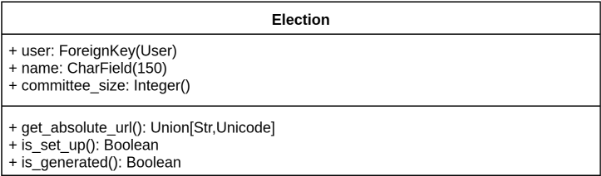
\includegraphics[scale=0.85]{pics/Election.png}}
\captionof{figure}{Obiekt mapowany na tabelę wyborów}
\end{center}
Pola:
\begin{itemize}
\item \code{user} - użytkownik aplikacji
\item \code{name} - nazwa wyborów
\item \code{committee\_size} - rozmiar zwycięskiego komitetu
\end{itemize}
Metody:
\begin{itemize}
\item \code{get\_absolute\_url()} - zwraca adres URL, który daje dostęp do danych wyborów z
poziomu dokumentu \textit{HTML}
\item \code{is\_set\_up()} - zwraca prawdę jeśli dla danych wyborów zostali określeni kandydaci i
głosujący lub fałsz w przeciwnym przypadku
\end{itemize}
\clearpage

\subsection{Candidate}
\begin{center}
\centerline{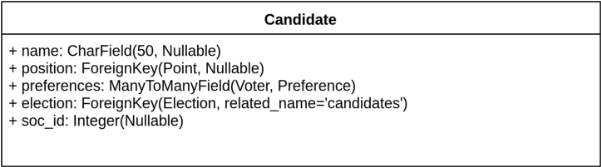
\includegraphics[scale=0.85]{pics/Candidate.png}}
\captionof{figure}{Obiekt mapowany na tabelę z danymi kandydata}
\end{center}
Pola:
\begin{itemize}
\item \code{name} - nazwa kandydata
\item \code{position} - położenie kandydata w układzie współrzędnych, pole opcjonalne dla
kandydatów generowanych z rozkładu normalnego
\item \code{preferences} - pole mapowane na relację wiele do wielu łączącej kandydata i
głosującego w tabeli \textit{Preference}
\item \code{election} - wybory, do których należy kandydat
\item \code{soc\_id} - identyfikator kandydata w odpowiadającym wyborom pliku w formacie \textit{.soc},
pole opcjonalne dla wyborów parsowanych z pliku
\end{itemize}

\subsection{Voter}
\begin{center}
\centerline{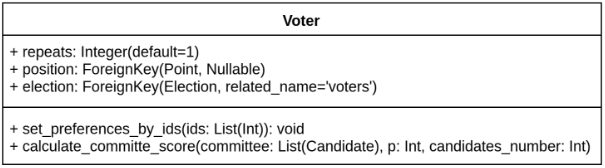
\includegraphics[scale=0.85]{pics/Voter.png}}
\captionof{figure}{Obiekt reprezentujący głos w wyborach}
\end{center}
Pola:
\begin{itemize}
\item \code{repeats} - liczba powtórzeń głosów w wyborach
\item \code{position} - współrzędne wyborcy na wykresie, pole opcjonalne, stosowane dla wyborów
generowanych z rozkładu normalnego
\item \code{election} - wybory, do których należy głosujący
\end{itemize}
\clearpage
Metody:
\begin{itemize}
\item \code{set\_preferences\_by\_ids()} - metoda wykorzystywana przy parsowaniu plików
w formacie \textit{.soc}.
Na podstawie ciągu identyfikatorów wyborców pobranego z pliku tworzy ciąg kandydatów ułożony według preferencji wyborcy. Pobrane dane zapisuje w bazie
danych w postaci rekordu w tabeli $Preference$.
\item \code{calculate\_committe\_score(committee: List(Candidate), \ p: Int, \
candidates\_number: Int)} - oblicza wynik komitetu \code{committee} na podstawie
parametru \code{p} i liczby kandydatów \code{candidates\_number}. Wynik mnożony jest przez
liczbę powtórzeń głosu.
\end{itemize}

\subsection{Preference}
\begin{center}
\centerline{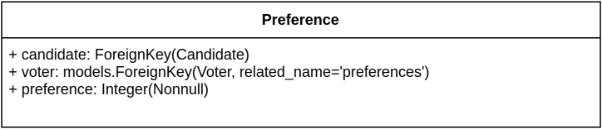
\includegraphics[scale=0.85]{pics/Preference.png}}
\captionof{figure}{Obiekt reprezentujący pozycję kandydata w liście preferencji głosującego}
\end{center}
Pola:
\begin{itemize}
\item \code{candidate} - kandydat związany z preferencją
\item \code{voter} - głosujący związany z preferencją
\item \code{preference} - pozycja preferencji na liście preferencji głosującego
\end{itemize}

\subsection{Point}
\begin{center}
\centerline{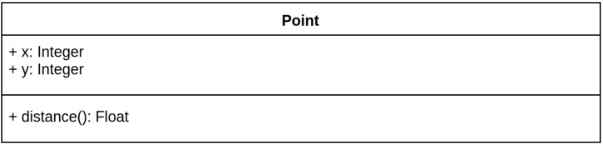
\includegraphics[scale=0.85]{pics/Point.png}}
\captionof{figure}{Obiekt przechowujący współrzędne wyborcy lub kandydata w układzie współrzędnych.}
\end{center}
\clearpage
Pola - współrzędne w układzie kartezjańskim:
\begin{itemize}
\item \code{x: Int}
\item \code{y: Int}
\end{itemize}
Metody:
\begin{itemize}
\item \code{distance(other: Point) : Float} - metoda zwracająca odległość punktu od punktu \code{other} w metryce euklidesowej w przestrzeni $R^2$
\end{itemize}

\subsection{Result}
\begin{center}
\centerline{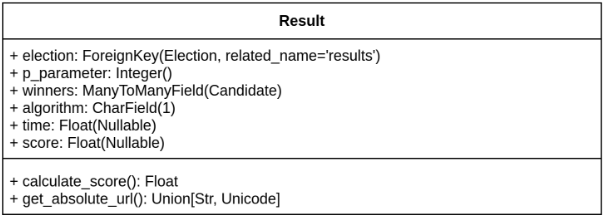
\includegraphics[scale=0.85]{pics/Result.png}}
\captionof{figure}{Obiekt mapowany na tabelę z danymi wyników wyborów: rodzaj algorytmu, parametry
wywołania algorytmu, otrzymany wynik punktowy komitetu oraz czas działania algorytmu}
\end{center}
Pola:
\begin{itemize}
\item \code{election} - wybory, dla których obliczono rezultat
\item \code{p\_parameter} - parametr $p$ normy $\ell_p$
\item \code{winners} - zwycięski komitet
\item \code{algorithm} - identyfikator algorytmu
\item \code{time} - czas wykonania obliczeń
\item \code{score} - wynik punktowy zwycięskiego komitetu
\end{itemize}

\clearpage
\subsection{GeneticAlgorithmSettings}
\begin{center}
\centerline{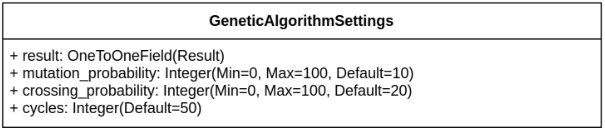
\includegraphics[scale=0.85]{pics/GeneticAlgorithmSettings.png}}
\captionof{figure}{Klasa mapowana na tabelę gromadząca dane specyficzne dla konfiguracji algorytmu
genetycznego. Wykorzystywana do zapisania specyficznych dla algorytmu genetycznego
parametrów wywołania.}
\end{center}
Pola:
\begin{itemize}
\item \code{result} - rezultat algorytmu genetycznego
\item \code{mutation\_probability} - prawdopodobieństwo wystąpienia mutacji danego osobnika
\item \code{crossing\_probability} - prawdopodobieństwo wymiany puli genów pomiędzy parą
osobników
\item \code{cycles} - liczba iteracji algorytmu genetycznego
\end{itemize}

\clearpage
\section{Diagram ERD}
\begin{center}
\centerline{\includegraphics[scale=0.45]{pics/ECS_ERD.png}}
\captionof{figure}{Diagram ERD}
\end{center}

\chapter{Algorytmy}
\section{Algorytm zachłanny}
\subsection{Idea algorytmu}
Idea algorytmu polega na dołączaniu kolejnego kandydata do zwycięskiego komitetu w
każdej iteracji. W związku z tym główna pętla algorytmu ma tyle iteracji, ile liczy rozmiar zwycięskiego komitetu. Jeżeli któryś z kandydatów został wybrany w danej iteracji jest
pewne, iż znajdzie się on w zwycięskim komitecie. Wybór kandydata w danej iteracji
dokonywany jest w sposób zachłanny. Spośród kandydatów, którzy jeszcze nie zostali
wybrani do zwycięskiego komitetu, dołącza do zwycięzców ten, który razem z wcześniej
wybranymi kandydatami tworzy komitet o największym uznaniu wśród wyborców. Mając
więc na danym etapie algorytmu komitet złożony z $k$ zwycięzców, w kolejnej iteracji
poszukiwany jest $k+1$-szy kandydat spośród pozostałych. Ma on stworzyć komitet liczący
$k+1$ członków, który jest najlepszy wśród wszystkich innych możliwości.W każdej iteracji
algorytmu wybierany jest kandydat, który najwięcej dodaje do aktualnego poziomu
zadowolenia wyborców. Stąd można uznać opisany algorytm jako zachłanny.

\subsection{Funkcja zadowolenia}
Aktualny poziom zadowolenia wyborców na danym etapie algorytmu określany jest za
pomocą uprzednio zdefiniowanego uogólnienia systemu $k-Borda$. Satysfakcja pojedynczego
wyborcy z komitetu liczącego na danym etapie algorytmu $k$ zwycięzców,określana jest za
pomocą funkcji: 
\begin{equation}
f_{{\ell_p}-Borda}(i_1, i_2,\dots, i_k) = \sqrt[p]{[\beta(i_1)]^p+[\beta(i_2)]^p+\dots+[\beta(i_k)]^p}
\end{equation}
 Funkcja bazuje na normie $\ell_p$ oraz punktacji $k-Borda$. Dokładne informacje na temat funkcji
umieszczone są w rozdziale \textit{Dziedzina problemu}. Ogólne zadowolenie wyborców z komitetu
jest obliczane jako suma pojedynczych zadowoleń wszystkich wyborców. Algorytm działa w
ten sposób, że przed wyborem pierwszego zwycięzcy, poziom zadowolenia wyborców
wynosi $0$, gdyż zadowolenie każdego pojedynczego wyborcy wynosi $0$ - zadowolenie z
komitetu liczącego $0$ osób zgodnie z powyższą funkcją wynosi $0$. W pierwszej iteracji
wybierany jest pierwszy zwycięzca w ten sposób, żeby suma pojedynczych zadowoleń
wszystkich wyborców z jednoosobowego komitetu była największa. W kolejnej iteracji
dobierany jest do wybranego wcześniej komitetu jednoosobowego drugi zwycięzca w ten
sposób, by suma pojedynczych zadowoleń wszystkich wyborców z dwuosobowego komitetu
była największa. W drugiej iteracji algorytmu brane więc pod uwagę są tylko wybrane
komitety dwuosobowe - takie, które składają się z wcześniej wybranego zwycięzcy i
dobranego wciąż jeszcze walczącego o zwycięstwo kandydata. W trzeciej iteracji do
wybranego wcześniej komitetu dwuosobowego dobierany jest trzeci zwycięzca w ten
sposób, by suma pojedynczych zadowoleń wszystkich wyborców z trzyosobowego komitetu
była największa. Podobnie jak w drugiej iteracji, pod uwagę brane są tylko wybrane komitety
trzyosobowe - takie, które składają się z wcześniej wybranego komitetu dwuosobowego i
dobranego wciąż jeszcze walczącego o zwycięstwo kandydata. W kolejnych iteracjach
algorytmu, kandydaci dobierani są w sposób analogiczny. Kandydaci dobierani są aż do
osiągnięcia określonego rozmiaru komitetu. Poziom zadowolenia wyborców po każdej
iteracji algorytmu rośnie.

\subsection{Szczegóły implementacji}
Algorytm zaimplementowany jest w klasie \code{GreedyAlgorithm} znajdującej się w pakiecie
\code{ecs.elections.algorithms.greedy\_algorithm}. Główna pętla algorytmu znajduje się w metodzie
\code{run()}. Przed główną pętlą programu do pamięci operacyjnej pobrane są obiekty z bazy danych
reprezentujące kandydatów, wyborców oraz preferencje wyborców. Ponadto odpowiednio
uzupełniane są struktury danych reprezentujące aktualne zadowolenie wyborców z wybranych kandydatów, aktualny skład zwycięskiego komitetu oraz kandydatów wciąż
walczących o zwycięstwo, którzy stanowią wszystkich kandydatów bez tych, którzy już
zostali wybrani do zwycięskiego komitetu. Początkowo poziom zadowolenia każdego
wyborcy wynosi $0$, skład zwycięskiego komitetu jest pusty, a kandydaci wciąż walczący o
zwycięstwo stanowią zbiór wszystkich kandydatów. \\ \\
W głównej pętli algorytmu znajdują się dwie wewnętrzne pętle. Bardziej zewnętrzna pętla
iteruje po wciąż walczących o zwycięstwo kandydatach, bardziej wewnętrzna pętla iteruje po
wszystkich wyborcach. Wskazane dwie wewnętrzne pętle mają na celu wyłonienie
najlepszego kandydata spośród jeszcze niewybranych kandydatów do zwycięskiego
komitetu. Dzieje się to poprzez obliczenie poziomu zadowolenia wyborców z komitetu
złożonego z kandydatów już wcześniej wybranych (na początku komitet zwycięski jest pusty)
wraz z dodatkowo dobranym kandydatem wcześniej niewybranym. Obliczany jest poziom
zadowolenia dla każdego możliwego dobrania (iteracja po kandydatach jeszcze
niewybranych) i ostatecznie w danej iteracji głównej pętli algorytmu do zwycięskiego
komitetu, dołączany jest kandydat, który wraz z wcześniej wybranymi kandydatami stanowi
największy poziom zadowolenia wyborców. W algorytmie najlepszy kandydat w danej iteracji
dobierany jest w ten sposób, że wskazany jest aktualny lider spośród kandydatów jeszcze
niewybranych wraz z poziomem satysfakcji wyborców z komitetu utworzonego z tego lidera i
z wcześniej wybranych kandydatów. Jeżeli poziom satysfakcji wyborców z komitetu z innym
niewybranym jeszcze kandydatem okaże się większy od tego z aktualnym liderem, aktualny
lider zostaje zmieniony a poziom satysfakcji zostaje aktualizowany. Ostatecznie w danej
iteracji głównej pętli algorytmu, do zwycięskiego komitetu dołączany zostaje lider po
zakończeniu iteracji po wszystkich jeszcze niewybranych kandydatach. Ponieważ poziom
zadowolenia z komitetu ustalany jest jako suma pojedynczych zadowoleń wszystkich
wyborców, w celu obliczenia funkcji satysfakcji dla komitetu złożonego z wcześniej
wybranych kandydatów wraz z dobranym kandydatem wcześniej niewybranym, następuje
iteracja po wszystkich wyborcach. Dla każdego wyborcy oceniane jest pojedyncze
zadowolenie z komitetu i dodawane do sumy zadowolenia wszystkich wyborców.
Pojedyncze zadowolenie liczone jest w ten sposób, że wyciągana jest punktacja badanego
kandydata według punktacji $k-Borda$, a następnie liczona jest norma $\ell_p$ z aktualnego
zadowolenia danego wyborcy (z wcześniej wybranych kandydatów) i punktów $k-Borda$
przyznanych dla badanego kandydata. Po wybraniu zwycięzcy, ostatnim krokiem w głównej
pętli algorytmu jest aktualizacja struktur danych reprezentujących aktualny stan algorytmu.
Do zwycięskiego komitetu zostaje dołączony wybrany w danej iteracji kandydat, przy
jednoczesnym usunięciu go ze zbioru kandydatów jeszcze niewybranych. Aktualizowane
zostają również pojedyncze satysfakcje wszystkich wyborców w oparciu o wybranego w
danej iteracji kandydata, który w tym momencie staje się zwycięzcą.

\subsection{Pseudokod}
%\begin{center}
% TODO poprawić znaczek różnicy w pseudokodzie
%\centerline{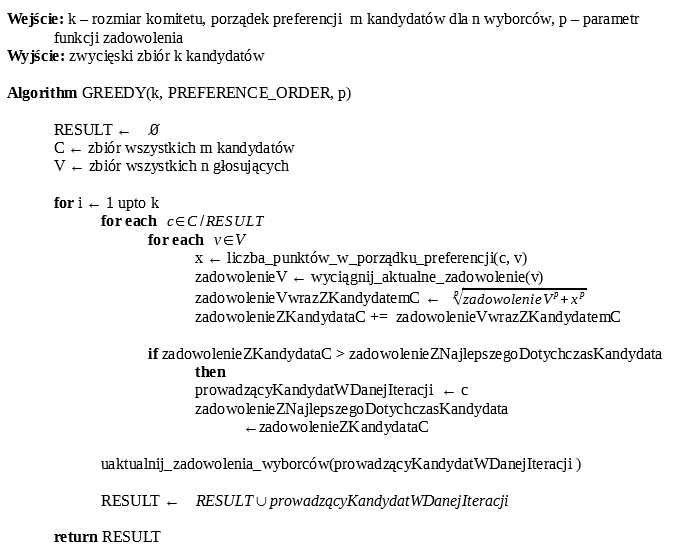
\includegraphics[scale=0.9]{pics/pseudocode_greedy_algorithm.png}}
%\captionof{figure}{Pseudokod algorytmu zachłannego}
%\end{center}
\begin{algorithm}[H]
\SetAlgoLined
\KwData{$k$ - rozmiar komitetu, $porzadek\_preferencji$ - porządek preferencji $m$ kandydatów dla $n$ wyborców, $p$ - parametr funkcji zadowolenia}
\KwResult{zwycięski zbiór $k$ kandydatów - zbiór $REZULTAT$}
$REZULTAT \longleftarrow \emptyset $ \;
$C \longleftarrow $ zbiór wszystkich $m$ kandydatów\;
$V \longleftarrow $ zbiór wszystkich $n$ wyborców\;
\For{$i \longleftarrow 1$ to $k$ }{
	\For{$c \in C\setminus REZULTAT$}{
		\For{$v \in V$}{
		$punkty\_Bordy \longleftarrow liczba\_punktow\_w\_porzadku\_preferencji(c, v, porzadek\_preferencji)$ \;
		$zadowolenie\_v \longleftarrow aktualne\_zadowolenie(v)$ \;
		$zadowolenie\_v\_wraz\_z\_kandydatem\_c \longleftarrow \sqrt[p]{zadowolenie\_v^p + punkty\_Bordy^p}$\;
		$zadowolenie\_z\_kandydata\_c += zadowolenie\_v\_wraz\_z\_kandydatem\_c$\;
		}
		\If{$zadowolenie\_z\_kandydata\_c > zadowolenie\_z\_najlepszego\_dotychczas\_kandydata$}{
		$prowadzacy\_kandydat\_w\_danej\_iteracji \longleftarrow c$\;
		$zadowolenie\_z\_najlepszego\_dotychczas\_kandydata \longleftarrow zadowolenie\_z\_kandydata\_c$\;
		}
		$uaktualnij\_zadowolenia\_wyborcow(prowadzacy\_kandydat\_w\_danej\_iteracji)$\;
		$REZULTAT \longleftarrow REZULTAT \cup prowadzacy\_kandydat\_w\_danej\_iteracji$\;
	}
}
\caption{Pseudokod algorytmu zachłannego}
\end{algorithm}


\section{Algorytm zachłanny według zasady Chamberlina-Couranta}
Algorytm ten nie aproksymuje wyników wyborów na bazie funkcji satysfakcji opisującej
system \mbox{$\ell_p-Borda$}, ale na szczególnym przypadku tej funkcji gdy $p \to \infty$. W związku z tym parametr $p$ nie wpływa na działanie algorytmu.

\subsection{Idea algorytmu}
Algorytm został zaproponowany przez Lu i Boutilier’a \footnote{E.Elkind, P.Faliszewski, P.Skowron. \textit{Properties of Multiwinner Voting Rule} - strona nr $6$}. Idea jest taka sama jak dla
pierwszego algorytmu zachłannego. W każdej iteracji głównej pętli algorytmu do
zwycięskiego komitetu dobrany zostaje jeden kandydat. Zwycięzca w danej iteracji zostaje
dobrany według postępowania zachłannego. Wygrywa kandydat, który najwięcej dodaje do
ogólnego poziomu zadowolenia wyborców. Różnica w stosunku do pierwszego algorytmu
zachłannego polega na innej funkcji zadowolenia, na bazie której inaczej obliczane są
pojedyncze zadowolenia wyborców i tym samym inaczej obliczane jest ogólne zadowolenie
wyborców z danego komitetu, które jest sumą pojedynczych satysfakcji wszystkich
wyborców. W regule \textit{Chamberlina-Couranta} położony jest nacisk na regułę reprezentacji proporcjonalnej. Każdy wyborca reprezentowany jest przez jednego, wyraźnego kandydata i
tylko punkty tego kandydata wpływają na wartość pojedynczego zadowolenia wyborcy z
danego komitetu. Jest to szczególny przypadek uogólnienia systemu $k-Borda$, w którym $p \to \infty$. Jednak dla odpowiednio dużych wartości parametru $p$ opisana heurystyka dobrze
sprawdza się dla uogólnienia systemu $k-Borda$.

\subsection{Funkcja zadowolenia}
Aktualny poziom zadowolenia wyborców na danym etapie algorytmu określany jest za
pomocą funkcji satysfakcji \textit{Chamberlina-Couranta}:
\begin{equation}
f_{CC}(i_1, i_2, ..., i_k) = \beta(i_1)
\end{equation}
Jest ona skrajnym przypadkiem dla uogólnienia systemu $k-Borda$, kiedy $p \to \infty$. Zgodnie z tą
funkcją, pojedyncze zadowolenie danego wyborcy z komitetu może wzrosnąć tylko w
przypadku, gdy do komitetu dołączany zostaje kandydat, któremu dany wyborca przydzielił
więcej punktów $k-Borda$ od punktów aktualnego reprezentanta. Jeżeli taki kandydat zostanie
dołączony do zwycięzców, to on staje się reprezentantem dla danego wyborcy w aktualnym
stanie algorytmu. Jest to odmienna sytuacja od pierwszego algorytmu zachłannego, w
którym pojedyncze zadowolenie danego wyborcy z komitetu rośnie wtedy, gdy nowo
dobrany kandydat ma jakiekolwiek przydzielone punkty $k-Borda$. W tamtym przypadku nowo
dołączony zwycięzca nie musi być najlepszy spośród wszystkich aktualnie wybranych
kandydatów do zwycięskiego komitetu, aby polepszyć indywidualne zadowolenie danego
wyborcy i tym samym zbiorcze zadowolenie wyborców.

\subsection{Szczegóły implementacyjne}
Algorytm zaimplementowany jest w klasie \code{GreedyCC} znajdującej się w pakiecie
\code{ecs.elections.algorithms.greedy\_cc}. Główna pętla algorytmu znajduje się w metodzie \code{run()}.
Implementacja i kolejne kroki algorytmu są takie same lub bardzo podobne jak dla
pierwszego algorytmu zachłannego zależnego od parametru $p$. Największa różnica jest w najbardziej wewnętrznej pętli
iterującej po wszystkich wyborcach. Zaimplementowana jest tu funkcja zadowolenia
pojedynczego wyborcy, różniąca się od analogicznej funkcji dla pierwszego algorytmu
zachłannego. Badany kandydat zwiększa wartość pojedynczej satysfakcji danego wyborcy
tylko wtedy, gdy ma on przydzielone u wyborcy najwięcej punktów $k-Borda$ w porównaniu z
dotychczasowymi zwycięzcami. W celu sprawdzenia czy potencjalny zwycięzca w danej
iteracji, zwiększa satysfakcję danego wyborcy, porównane są dwie wartości: punkty $k-Borda$
przyznane przez wyborcę dla potencjalnego zwycięzcy i punkty $k-Borda$ przyznane przez
wyborcę dla najlepszego spośród kandydatów aktualnego zwycięskiego komitetu. Jeśli
punkty dla badanego kandydata są większe od punktów najlepszego dotychczasowego
zwycięzcy, dodatkowa satysfakcja dla badanego kandydata od danego wyborcy jest
uzupełniania o różnicę między punktami $k-Borda$ przydzielonymi dla badanego kandydata i
punktami $k-Borda$ przydzielonymi dla najlepszego dotychczas kandydata. W danej iteracji
wygrywa kandydat, który wniósł najwięcej dodatkowej satysfakcji do ogólnego zadowolenia
wyborców. Drugą istotną różnicą wspomnianą przy omawianiu pierwszej, jest sposób
porównania w danej iteracji niewybranych jeszcze kandydatów w celu ustalenia najlepszego
z nich. Polega on na zbadaniu jaką dodatkową satysfakcję do ogólnego poziomu
zadowolenia wnosi badany kandydat i porównywaniu tych dodatkowych satysfakcji, a nie
wartości ogólnego poziomu zadowolenia jak w przypadku pierwszego algorytmu.

\section{Algorytm genetyczny}
Algorytmy genetyczne polegają na przedstawieniu róznych wyników problemu 
jako \textit{osobników}, a następnie, w sposób losowy, ich krzyżowanie i mutowanie. 
Po każdym takim cyklu osobniki są poddawane ocenie i do dalszych cykli pozostawiane są tylko
najlepsze okazy. Algorytm opiera się na znanej z biologii ewolucji.

\subsection{Osobnik}
W naszej implementacji osobnikiem jest wybierany komitet (podzbiór kandydatów). 
Po utworzeniu jest on oceniany według funkcji satysfakcji i przypisywany jest mu wynik.

\subsection{Krzyżowanie}
Krzyżowanie osobników - komitetów polega na losowym wybraniu kandydatów z dwóch osobników, tak by łącznie było ich $k$ i żaden się nie powtarzał (krzyżowane osobniki mogą zawierać tych samych kandydatów).

\subsection{Mutacja}
Mutacja osobnika - komitetu polega na losowej zmianie jednego z kandydatów z komitetu na innego, wcześniej niewybranego.

\subsection{Parametry algorytmu}
System pozwala wybrać:
\begin{itemize}
\item liczbę cykli działania algorytmu
\item cześć puli jaka jest poddawana krzyżowaniu (osobniki są z niej losowo wybierane do krzyżowania)
\item prawdopodobieństwo wystąpienia mutacji w pojedynczym osobniku
\end{itemize}

\subsection{Cykl algorytmu}
Na cykl algorytmu składa się:
\begin{itemize}
\item wybór par osobników do krzyżowania się
\item krzyżowanie osobników
\item mutacja osobników zgodnie z zadanym prawdopodobieństwem
\item wybór N osobników do przejścia do kolejnego cyklu
\end{itemize}

Liczba N określa wielkość puli osobników i jest wybierana na początku działania algorytmu. W naszej implementacji przyjęto stałą liczbę 50 osobników.

\subsection{Wpływ parametrów działania na wyniki osiągane przez algorytm}
Aby przekonać się jak dobór parametrów ma wpływ na wyniki osiągane przez algorytm, przeprowadzono kilka testów na losowo wygenerowanych wyborach (korzystając z funkcji systemu losującej kandydatów i wyborców na podstawie rozkładu normalnego).

Dla przykładu - dla wyborów $20$ spośród $100$ kandydatów, przy $100$ wyborcach, czasy działania algorytmu wahały się w zakresie od $4,3s$ do $150,3$s. Przy czym wyniki różniły się również znacząco - komitety uzyskiwały od $10715,65$ do $10867,96$ punktów. W tej serii zostały przetestowane wszystkie kombinacje parametrów spośród następujących:

$\textit{liczba cykli} \in \{ 20, 50, 100 \}$

$\textit{prawdopodobieństwo mutacji} \in \{ 10\%, 25\%, 50\% \}$

$\textit{krzyżowanie} \in \{ 10\%, 50\%, 100\% \}$

~\\ 
Okazuje się jednak, że nawet te parametry nie wystarczają do wyznaczenia najlepszego wyniku - obliczenia w $200$ cyklach (z prawdopodobieństwem mutacji $50\%$ i krzyżowaniem całej puli) dały jeszcze wyższy wynik - $10868.15$, przy czasie $364s$. 

Należy mieć na uwadze, że w działaniu algorytmu genetycznego wiele zależy od udziału czynnika losowego i wyniki są tym obarczone.

\newpage

Poniżej znajdują się wykresy obrazujące czas i wyniki osiągane przez algorytm genetyczny dla tego zestawu danych przy różnych parametrach:

\begin{tabular}{cc}
	
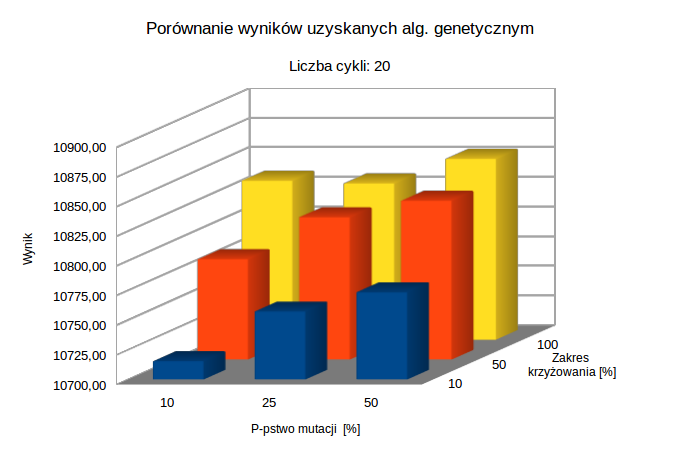
\includegraphics[width=0.4\paperwidth]{pics/porownanie1/wynik20.png} & 
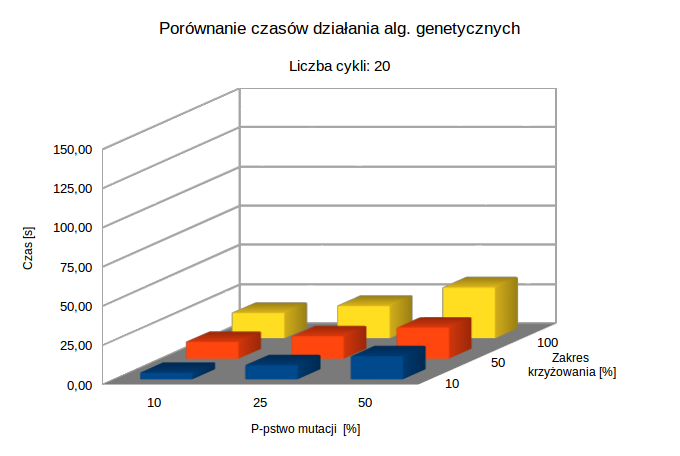
\includegraphics[width=0.4\paperwidth]{pics/porownanie1/czas20.png} \\
	
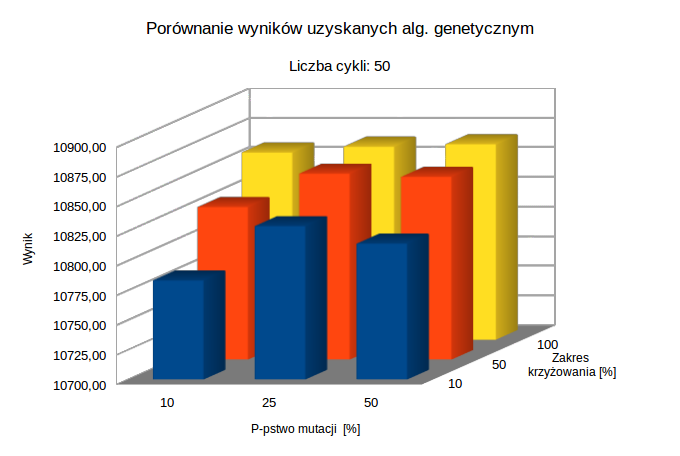
\includegraphics[width=0.4\paperwidth]{pics/porownanie1/wynik50.png} & 
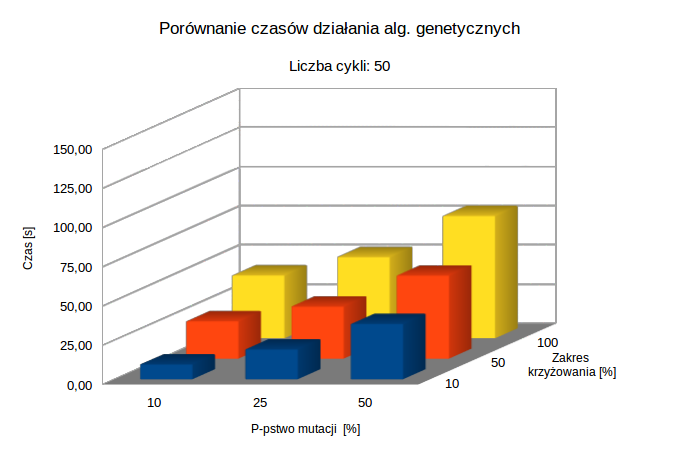
\includegraphics[width=0.4\paperwidth]{pics/porownanie1/czas50.png} \\
	
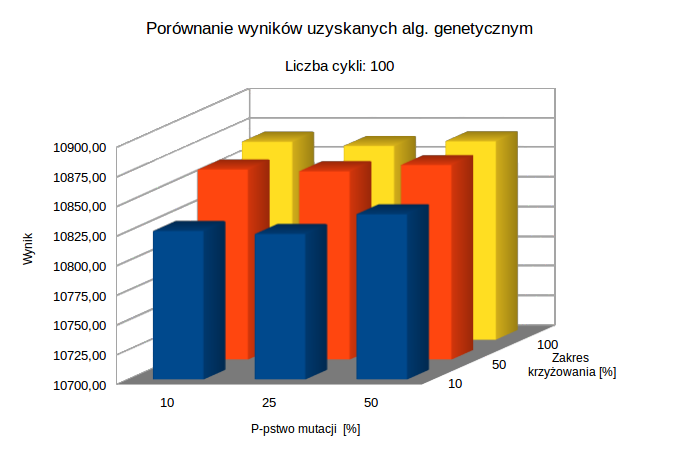
\includegraphics[width=0.4\paperwidth]{pics/porownanie1/wynik100.png} & 
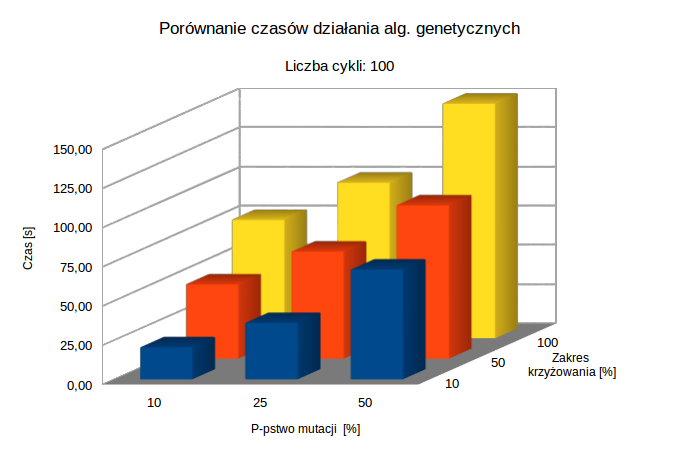
\includegraphics[width=0.4\paperwidth]{pics/porownanie1/czas100.png} \\
		
\end{tabular}
\captionof{figure}{Porównanie wyników i czasów działania algorytmu genetycznego z różnymi parametrami}

\newpage

Należy pamiętać, że nawet mała zmiana wyniku punktowego komitetu może mieć duży wpływ na faktycznie wybranych kandydatów - poniżej znajdują się mapy preferencji z zaznaczonymi dwoma wybranymi komitetami, których wynik różni się zaledwie o około $19$ setnych punktu. Są to dwa najlepsze rezultaty wspomniane wcześniej.

\begin{center}
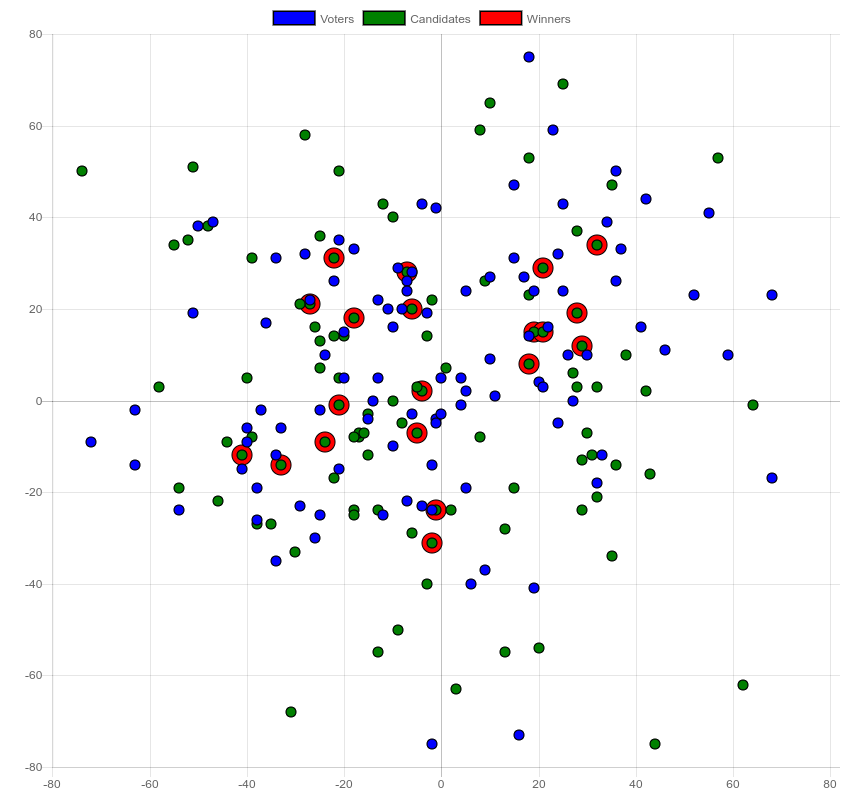
\includegraphics[width=0.5\paperwidth]{pics/porownanie1/wynik1.png} 
\captionof{figure}{Wybrany w $150,29s$ komitet o punktacji $10867,96$}


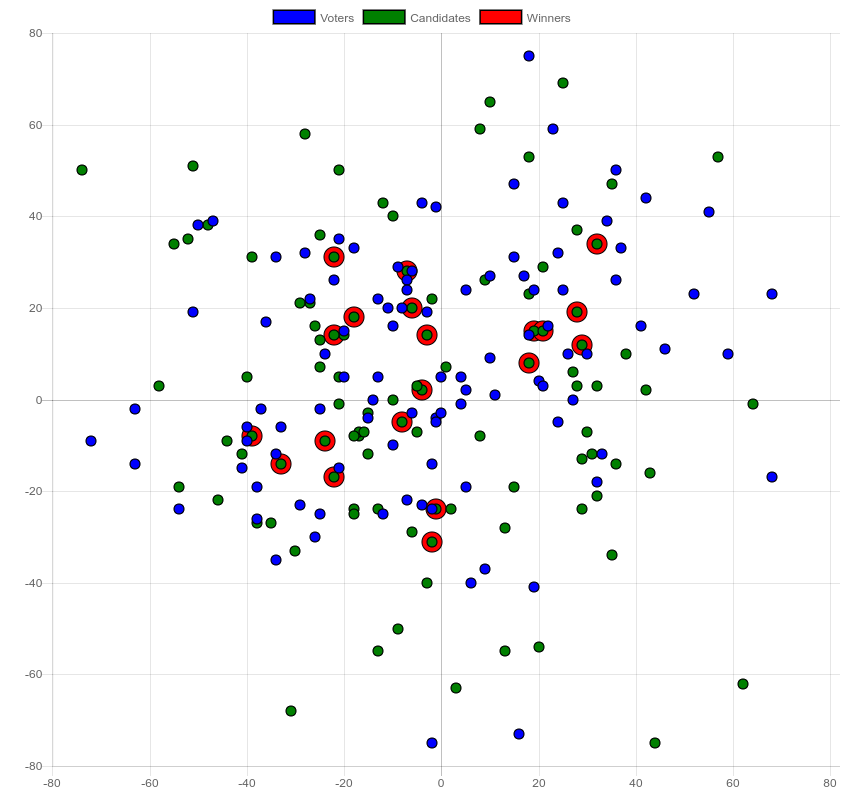
\includegraphics[width=0.5\paperwidth]{pics/porownanie1/wynik2.png}
\captionof{figure}{Wybrany w $363,92s$ komitet o punktacji $10868,15$}
\end{center}

\newpage

Podobne zestawienie wykonano jeszcze dla "większych" wyborów: $200$ głosujących, $200$ kandydatów, $15$ miejsc w komitecie. Poniżej znajduje się porównanie osiągniętych wyników:

\begin{tabular}{cc}
	
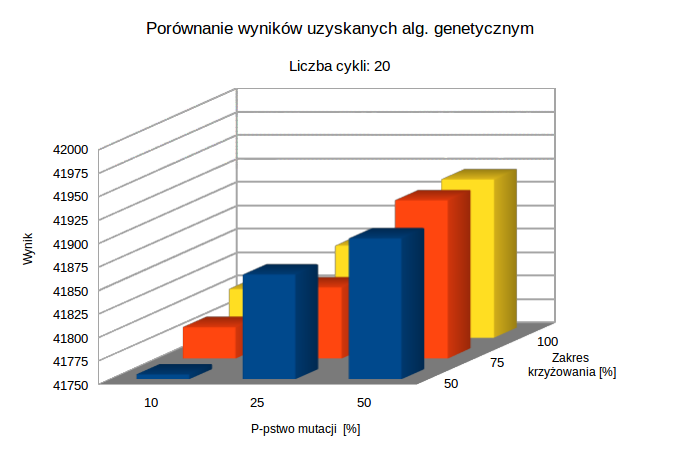
\includegraphics[width=0.4\paperwidth]{pics/porownanie2/wynik20.png} & 
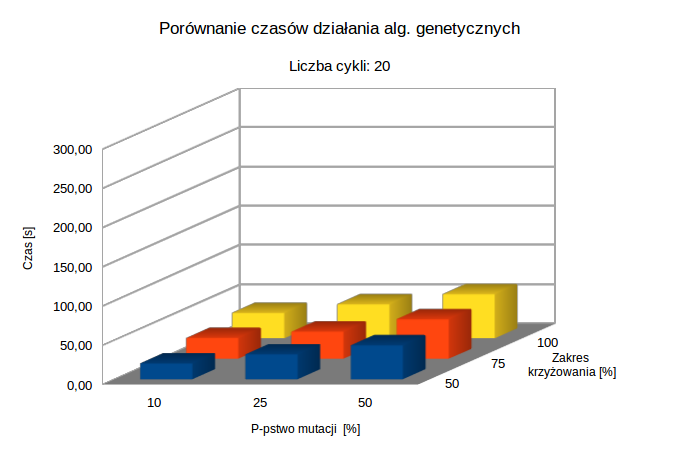
\includegraphics[width=0.4\paperwidth]{pics/porownanie2/czas20.png} \\
	
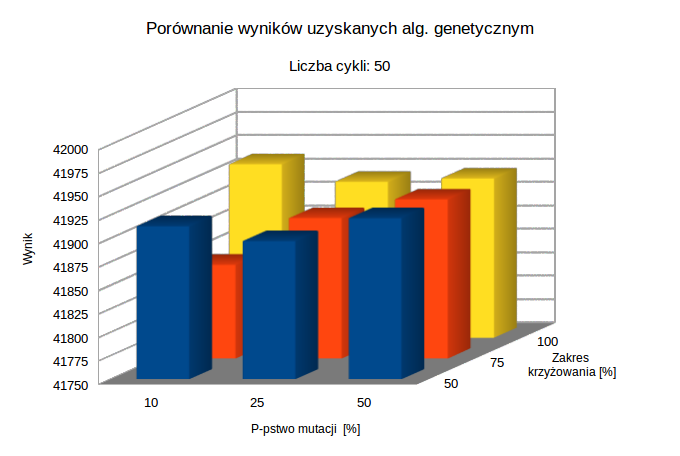
\includegraphics[width=0.4\paperwidth]{pics/porownanie2/wynik50.png} & 
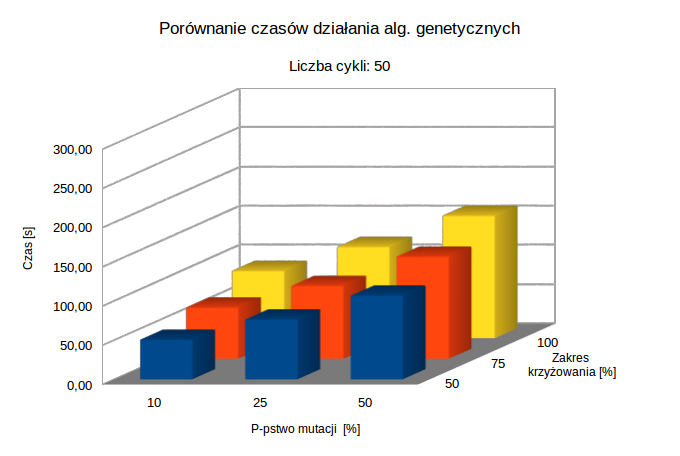
\includegraphics[width=0.4\paperwidth]{pics/porownanie2/czas50.png} \\
	
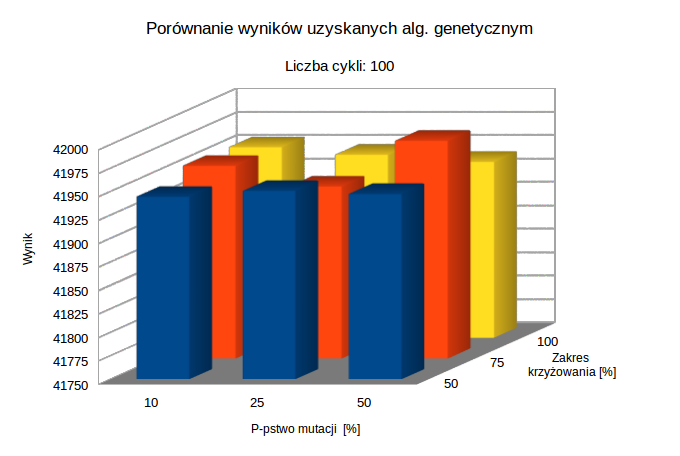
\includegraphics[width=0.4\paperwidth]{pics/porownanie2/wynik100.png} & 
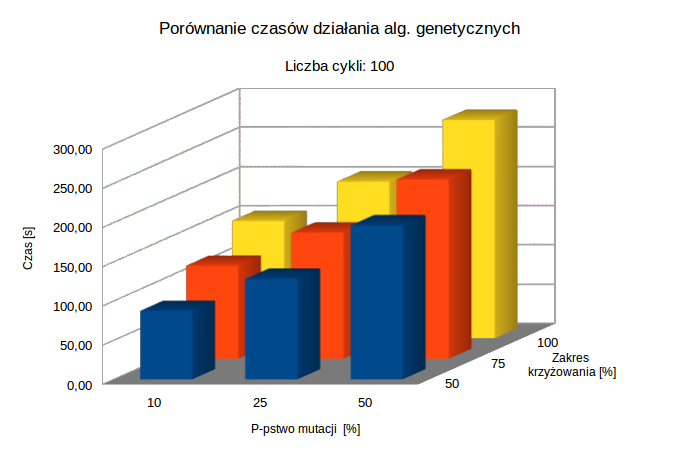
\includegraphics[width=0.4\paperwidth]{pics/porownanie2/czas100.png} \\
		
\end{tabular}
\captionof{figure}{Porównanie wyników i czasów działania algorytmu genetycznego z różnymi parametrami}

~ \\
W tym wypadku również zwiększenie liczby cykli do $200$ pozwoliło na jeszcze lepszy wynik, windując jednak czas wykonania programu do nieco ponad $10$ minut. Co ciekawe próba przy $300$ cyklach dała wynik gorszy - ujawnia się tutaj losowa natura algorytmu genetycznego.

\section{Algorytm typu brute-force}
Do zbadania poprawności działania innych algorytmów zaimplementowany został bardzo prosty algorytm typu \textit{brute-force} iterujący po wszystkich możliwych kombinacjach komitetów i wyszukujący komitetu o najwyższym wyniku.

\subsection{Pseudokod}

\begin{algorithm}[H]
\SetAlgoLined
\KwData{$K$ - zbiór wszystkich możliwych komitetów w danych wyborach}
\KwResult{$REZULTAT$ - zwycięski zbiór $k$ kandydatów}
~\\
$REZULTAT \longleftarrow \emptyset $ \\
$najlepszy\_wynik \longleftarrow $ 0 \\
\For{$k \in K$ }{ ~\\
	\If{$wynik(k) > najlepszy\_wynik$}{ ~\\
		$REZUTLAT \longleftarrow k$ \\
		$najlepszy\_wynik \longleftarrow wynik(k)$
	}
}
\caption{Pseudokod algorytmu \textit{brute-force}}
\end{algorithm}


\chapter{Porównanie algorytmów}
\section{Zrównanie jakości działania algorytmów zachłannych}
Ponieważ algorytm zachłanny według zasady \textit{Chamberlina-Couranta} przystosowany jest do
działania dla dużych wartości parametru $p$ (im większy parametr $p$, tym wartość wskazanego przez algorytm komitetu powinna rosnąć), zasadnym jest analiza dla jakiego parametru $p$ algorytm zachłanny
według zasady \textit{Chamberlina-Couranta} staje się nie gorszy od algorytmu zachłannego zależnego
od parametru $p$. Algorytm zachłanny według zasady \textit{Chamberlina-Couranta} jest znacznie szybszy od swojego konkurenta, więc wiedząc dla jakiej wartości parametru $p$ staje się nie gorszy pod względem jakości rezultatu, można go z powodzeniem stosować zamiast algorytmu zachłannego zależnego od parametru $p$. W tym podrozdziale podjęta zostanie próba oszacowania wartości parametru $p$, dla którego algorytmy zachłanne zrównują się pod względem jakości wyniku oraz zostanie przeprowadzona analiza czynników, które mogą potencjalnie wpływać na wartość tego parametru $p$. W dalszej części podrozdziału parametr $p$, dla którego algorytmy zachłanne zrównują się pod względem jakości wyniku będzie nazywany graniczną wartością parametru $p$.
\subsection{Działanie algorytmów zachłannych}
Dla wszystkich przypadków testowanych, wyniki algorytmów zachłannych zachowywały pewien schemat wraz ze wzrostem parametru $p$. Dla małych wartości parametru $p$ jakość rezultatu obliczonego przez algorytm zachłanny zależny od wartości parametru $p$, znacznie przewyższa drugi z algorytmów zachłannych. Wraz ze wzrostem parametru $p$ jakości wyników wyliczanych przez algorytmy są coraz bliższe sobie. Dla pewnej wartości granicznej parametru $p$, algorytm zachłanny według zasady
\textit{Chamberlina-Couranta} staje się nie gorszy od swojego konkurenta pod względem jakości
wyniku. Dla wartości parametru $p$ większych od tej wartości granicznej, algorytm zachłanny według zasady
\textit{Chamberlina-Couranta} jest co najmniej tak samo dobry jak algorytm zachłanny zależny od
parametru $p$. Dla wartości parametru $p$ większych i równych od wartości granicznej parametru $p$, najczęściej występuje taka sytuacja, że wyniki obydwu algorytmów są takie same.

Powyższa zasada zachowywania się wyników algorytmów zachłannych względem siebie sprawdziła się dla wszystkich przypadków testowanych. Ponieważ badane algorytmy są algorytmami heurystycznymi, mogą wystąpić odstępstwa od tej reguły.

\subsection{Wpływ liczby wyborców na wartość graniczną parametru $p$}
Pierwszym czynnikiem, który badano pod kątem jego wpływu na wartość graniczną parametru $p$, była liczba wyborców. W tym celu określono pewne stałe wartości dla innych parametrów definiujących wybory, a następnie szacowano wartość graniczną parametru $p$. Szacowanie polegało na poszukiwaniu wartości granicznej w ten sposób, że porównywano dla pewnej wybranej początkowo wartości parametru $p$ wyniki obydwu algorytmów i w zależności, który algorytm okazał się lepszy pod względem jakości wyniku, dalsze poszukiwanie ograniczano do wartości parametru $p$ mniejszych lub większych wybranej początkowo wartości. Jeżeli lepszy okazywał się algorytm zachłanny zależny od wartości parametru $p$, wtedy dalsze poszukiwanie ograniczano do wartości parametru $p$ większych od badanej początkowo wartości parametru $p$. W przeciwnym przypadku szukano dla wartości parametru $p$ mniejszych od wybranej na początku wartości. Postępowanie w celu oszacowania wartości granicznej parametru $p$ miało cechy wyszukiwania binarnego. Wartość graniczna parametru $p$ nie była określana dokładnie, lecz jedynie szacowana. Błąd bezwzględny określonej wartości wynosił dla tego testu $50$. Jeżeli przykładowo stwierdzono, że wartość graniczna znajduje się między wartością $1500$ a $1600$, to szacowano, że wartość graniczna parametru $p$ wynosi $1550$. Dla tego testu przyjęto, że rozmiar komitetu będzie wynosił $15$, a liczba kandydatów będzie wynosiła $50$. Zbadano zależność wartości granicznej parametru $p$ dla liczby wyborców wynoszącej $25$, $50$, $75$ oraz $100$. Próbę przeprowadzono dwukrotnie dla każdej wartości liczby wyborców w celu określenia czy wynik dla danej liczby wyborców jest podobny niezależnie od innych parametrów. Testy przeprowadzano dla wyborów generowanych z rozkładu normalnego. Wyniki przedstawione są w formie tabeli i wykresu. \\

\begin{center}

\begin{tabular}{|c|c|c|c|c|}
   \hline
   liczba wyborców & 25 & 50 & 75 & 100 \\
   \hline
   wartość graniczna parametru $p$ - próba nr 1 & 1550 & 1600 & 50 & 100 \\
   \hline
   wartość graniczna parametru $p$ - próba nr 2 & 50 & ponad 5000 & 1150 & 50 \\
   \hline
\end{tabular}
\captionof{table}{Graniczne wartości parametru $p$ dla różnej liczby wyborców}
\end{center}

\vspace{\baselineskip}

\begin{center}
\centerline{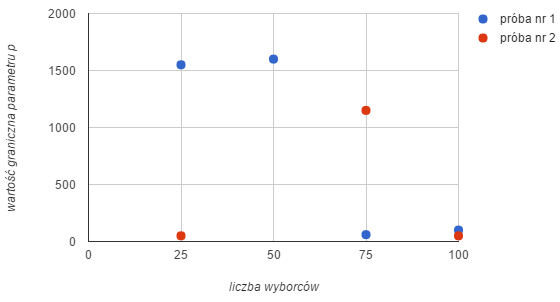
\includegraphics[scale=1]{pics/wartosc_graniczna_od_liczba_wyborcow.png}}
\captionof{figure}{Zależność wartości granicznej parametru $p$ od liczby wyborców}
\end{center}

Na wykresie nie zaznaczono wyniku drugiej próby dla liczby wyborców równej $50$. Nie oszacowano jej dokładnie, gdyż wiadomo że wynosiła ponad $5000$. Nie jest istotne jak duża jest ta wartość. Badanie to pokazało, że nie ma zależności między wartością graniczną parametru $p$ a liczbą wyborców. Rozrzut wyników jest bardzo duży nawet dla dwóch różnych prób dla tej samej liczby wyborców.

\subsection{Wpływ odchylenia standardowego na wartość graniczną parametru $p$}
Zdecydowano się na sprawdzenie wpływu rozproszenia wyborców i kandydatów na wartość graniczną parametru $p$. Wartości parametru były takie same jak w poprzednim teście poza wartością odchylenia standardowego. Wcześniej wartość odchylenia standardowego dla wyborców i kandydatów wynosiła domyślne $30$. W tym teście podniesiono tą wartość do $100$. Sposób przeprowadzenia testu był analogiczny do poprzedniego. Wyniki przedstawione są w formie tabeli.

\begin{center}
\begin{tabular}{|c|c|c|}
   \hline
   liczba wyborców & 25 & 50 \\
   \hline
   wartość graniczna parametru $p$ - próba nr 1 & ponad 5000 & 1500 \\
   \hline
   wartość graniczna parametru $p$ - próba nr 2 & 50 & 50 \\
   \hline
\end{tabular}
\captionof{table}{Graniczne wartości parametru $p$ dla różnej liczby wyborców i $\sigma = 100$}
\end{center}

Ponieważ po dwukrotnym sprawdzeniu wyniku dla dwóch różnych liczb wyborców, rozrzut wyników okazał się równie duży jak w przypadku pierwszego testu, stąd poprzestano na tych wynikach. Wpływu odchylenia standardowego w ten sposób badanego na graniczną wartość parametru $p$ nie odnotowano.

\subsection{Wpływ liczby kandydatów na wartość graniczną parametru $p$}
Kolejnym zbadanym czynnikiem był wpływ liczby kandydatów na wartość graniczną parametru $p$ przy założeniu, że pozostałe parametry definiujące wybory są stałe. Na potrzeby testu przyjęto, że rozmiar komitetu będzie równy $15$, liczba wyborców wyniesie $50$, a odchylenie standardowe zarówno dla wyborców, jak i kandydatów wyniesie domyślne $30$. Sposób przeprowadzenia testu był analogiczny do poprzednich. Błąd bezwzględny oszacowanych wartości granicznych, dla wartości rzędu kilku tysięcy wynosił $250$, dla rzędu kilkaset lub kilkadziesiąt $50$. Jeżeli przykładowo stwierdzono, że wartość graniczna znajduje się między wartością $3000$ a $3500$, to szacowano, że wartość graniczna parametru $p$ wynosi $3250$. Większa dokładność okazała się nieistotna. Wyniki przedstawione są w formie tabeli.

\begin{center}
\begin{tabular}{|c|c|c|}
   \hline
   liczba kandydatów & 20 & 40 \\
   \hline
   wartość graniczna parametru $p$ - próba nr 1 & 850 & 3250 \\
   \hline
   wartość graniczna parametru $p$ - próba nr 2 & 250 & 50 \\
   \hline
\end{tabular}
\captionof{table}{Graniczne wartości parametru $p$ dla różnej liczby kandydatów}
\end{center}

Ponieważ podobnie jak w poprzednim teście rozrzut wyników okazał się bardzo duży, zdecydowano poprzestać na dwukrotnym sprawdzeniu dwóch różnych liczb kandydatów. Dla takiej samej liczby kandydatów, wartość graniczna parametru $p$ potrafi być jednocześnie i bardzo duża i bardzo mała. Wpływu w ten sposób badanej liczby kandydatów na graniczną wartość parametru $p$ nie znaleziono.

\subsection{Wpływ rozmiaru komitetu na wartość graniczną parametru $p$}
Kolejnym badanym czynnikiem był rozmiar komitetu. Metodyka badania była taka sama jak w poprzednim teście. Błąd bezwzględny oszacowanych wartości granicznych, dla wartości rzędu kilku tysięcy wynosił $500$, dla rzędu kilkaset lub kilkadziesiąt $50$. Parametry definiujące wybory poza rozmiarem komitetu przyjęto jako stałe. Liczbę kandydatów określono na wartość $60$, liczbę wyborców na 50, a odchylenie standardowe wyborców i kandydatów na domyślne $30$. Wyniki przedstawiono w formie tabeli i wykresu.

\begin{center}
\begin{tabular}{|c|c|c|c|c|c|}
   \hline
   rozmiar komitetu & 10 & 20 & 30 & 40 & 50 \\
   \hline
   wartość graniczna parametru $p$ - próba nr 1 & 50 & 2500 & 4000 & 3500 & 3500 \\
   \hline
   wartość graniczna parametru $p$ - próba nr 2 & 100 & 1500 & 3500 & 3500 & 3000 \\
   \hline
\end{tabular}
\captionof{table}{Graniczne wartości parametru $p$ dla różnego rozmiaru komitetu}
\end{center}

\vspace{\baselineskip}

\begin{center}
\centerline{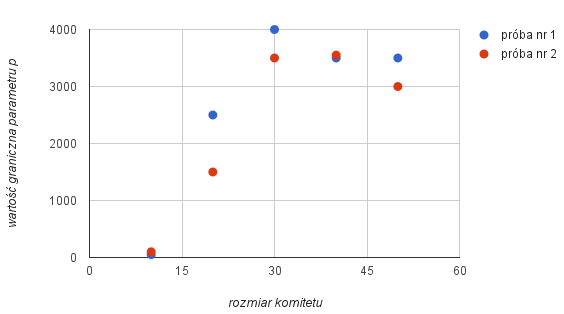
\includegraphics[scale=1]{pics/wartosc_graniczna_od_rozmiar_komitetu.png}}
\captionof{figure}{Zależność wartości granicznej parametru $p$ od rozmiaru komitetu}
\end{center}

Rozrzut wyników dwóch różnych prób dla badanych rozmiarów komitetów był w porównaniu do poprzednich badań stosunkowo niewielki. Dla najmniejszego rozmiaru komitetu wynoszącego $10$, wartość graniczna parametru $p$ była rzędu kilkadziesiąt. Dla rozmiaru komitetu równego $20$ rozrzut wyników był największy. Dla większych rozmiarów komitetu wartość graniczna była na poziomie kilka tysięcy i zdawała się mieć pewien rodzaj stabilizacji. Wciąż jednak trudno stwierdzić czy istnieje jakakolwiek zależność między badanymi wielkościami. Można jedynie zaobserwować, że dla mniejszych rozmiarów komitetu wartość graniczna przybiera dość często małą wartość rzędu kilkadziesiąt, a dla większych rozmiarów komitetu wartość graniczna jest raczej rzędu kilka tysięcy.

Przeprowadzając wszystkie powyższe testy zauważono jednak inną prawidłowość. Otóż zaobserwowano, że już dla niewielkiej wartości parametru $p$ większość zwycięzców wskazanych przez obydwa algorytmy pokrywa się ze sobą. O innej wartości wskazanego komitetu dla większych wartości parametru $p$ decyduje niewielka część zwycięzców. Tworzą się pary lub trójki kandydatów, którzy znajdują się blisko siebie i w zależności od tego który z nich zostanie wybrany do zwycięskiego komitetu, wartości zadowolenia wyborców się nieco zmieniają. Przykładowo może się tak zdarzyć, że istnieje para kandydatów spośród której zawsze do zwycięskiego komitetu trafia jeden z kandydatów w tej parze. Przy czym istnieje graniczna wartość parametru $p$, poniżej której zawsze jeden z kandydatów w tej parze wchodzi do zwycięskiego komitetu i jednocześnie powyżej tej granicznej wartości parametru $p$ drugi kandydat z pary wchodzi do zwycięskiego komitetu. Jeżeli ta graniczna wartość jest duża, to wtedy algorytm zachłanny zależny od parametru $p$ długo będzie wybierał pierwszego kandydata z pary
przewyższając tym samym algorytm według zasady \textit{Chamberlina-Couranta}, który zawsze wybierze drugiego
kandydata. Stąd graniczna wartość parametru $p$ dla tego przypadku jest duża, bo algorytm zachłanny zależny od parametru $p$ będzie długo minimalnie lepszy od drugiego algorytmu zachłannego. Jednak trzon zwycięzców dla obydwu algorytmów szybko jest taki sam. Stąd na wartość graniczną parametru $p$ głównie ma wpływ lokalne rozmieszczenie kandydatów. Jeżeli znajdą się pary i trójki, spośród których dla dużych wartości parametru $p$ następuje zamiana miejsc w zwycięskim komitecie, wtedy wartość graniczna parametru $p$ jest dla takich przypadków duża. Jeżeli takich zaciętych par nie ma i zwycięzcy są wyłaniani w zdecydowany sposób pod kątem reprezentatywności dla pewnej części wyborców, wtedy wartość graniczna parametru $p$ jest mała. Poniekąd taka interpretacja tłumaczy tendencję do małej wartości granicznej parametru $p$ dla małych zwycięskich komitetów i dużą wartość graniczną parametru $p$ dla dużych zwycięskich komitetów. Dla małych rozmiarem komitetów, każdy ze zwycięzców klarownie reprezentuje pewną część wyborców przez co nie tworzą się dla większych $p$ pary rywalizujące o reprezentację dla pewnej części wyborców. Dla dużych komitetów, w związku z wieloma miejscami w komitecie o zwycięstwo rywalizują również mniej popierani w danej grupie wyborców kandydaci, przez co jest większa szansa na stworzenie się opisanej wcześniej pary lub trójki kandydatów.

\subsection{Stopień pokrywania się zwycięzców dla różnych wartości parametru p}
W związku z zaobserwowaniem faktu dużego pokrywania się zwycięskich kandydatów wyłanianych przez algorytmy zachłanne dla odpowiednio dużych wartości parametru $p$, postanowiono dokładniej zbadać tę kwestię. Sprawdzono jaki procent kandydatów ze zwycięskich komitetów wyłonionych przez obydwa algorytmy pokrywa się ze sobą. Testy przeprowadzono dla różnych wartości definiujących wybory. Dla każdej ze sprawdzonych wartości parametru $p$ sprawdzono pokrycie się zwycięzców dla $10$ różnych wyborów. Dla każdej wartości parametru $p$ policzono następnie średnią i medianę z wyliczonych wartości procentowych pokrycia się komitetów. Wyniki poszczególnych prób i obliczonych średnich oraz median przedstawiono w formie tabeli. W tabeli przyjęto następujące oznaczenia: $k$ - rozmiar komitetu, $c$ - liczba kandydatów, $v$ - liczba wyborców. Dla poszczególnych wyborów przedstawiono ilu zwycięskich kandydatów z całego komitetu pokryło się z wynikami drugiego algorytmu dla danej wartości parametru $p$. Średnie i mediany przedstawiono również w formie wykresu.

%\clearpage
\begin{center}
\begin{tabular}{|c|c|c|c|c|}
\hline 
parametr $p$ & 30 & 50 & 100 & 1000 \\ 
\hline 
$k$ = 10, $c$ = 70, $v$ = 100 & 6/10 & 8/10 & 8/10 & 9/10 \\ 
\hline 
$k$ = 15, $c$ = 55, $v$ = 75 & 13/15 & 15/15 & 15/15 & 15/15 \\ 
\hline 
$k$ = 20, $c$ = 50, $v$ = 40 & 15/20 & 15/20 & 15/20 & 17/20 \\ 
\hline 
$k$ = 25, $c$ = 65, $v$ = 80 & 20/25 & 23/25 & 24/25 & 24/25 \\ 
\hline 
$k$ = 30, $c$ = 80, $v$ = 45 & 26/30 & 26/30 & 27/30 & 27/30 \\ 
\hline 
$k$ = 35, $c$ = 45, $v$ = 75 & 30/35 & 34/35 & 34/35 & 34/35 \\ 
\hline 
$k$ = 40, $c$ = 75, $v$ = 60 & 35/40 & 35/40 & 36/40 & 36/40 \\ 
\hline 
$k$ = 45, $c$ = 85, $v$ = 50 & 38/45 & 40/45 & 41/45 & 41/45 \\ 
\hline 
$k$ = 50, $c$ = 150, $v$ = 150 & 34/50 & 39/50 & 46/50 & 47/50 \\ 
\hline 
$k$ = 55, $c$ = 95, $v$ = 110 & 44/55 & 49/55 & 54/55 & 54/55 \\ 
\hline 
średnia & 79.4 \% & 87.43 \% & 90.94 \% & 93.14 \% \\ 
\hline 
mediana & 82.22 \% & 88.19 \% & 91.55 \% & 92.55 \% \\ 
\hline 
\end{tabular}
\captionof{figure}{Procentowe pokrycie się zwycięskich kandydatów dla różnych wartości parametru $p$} 
\end{center}

\vspace{\baselineskip}

\begin{center}
\centerline{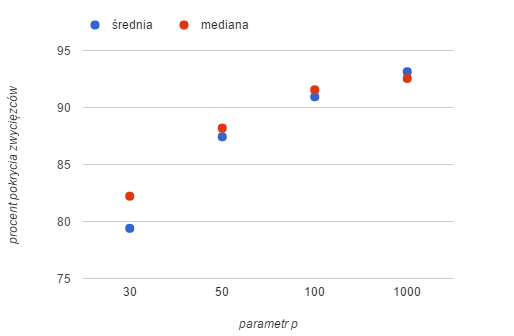
\includegraphics[scale=1]{pics/srednia_mediana_od_parametr_p.png}}
\captionof{figure}{Średnie i mediany pokrycia się zwycięskich komitetów}
\end{center}

Uzyskane wyniki pokazują, że już dla wartości parametru $p = 50$ średnio ponad $87 \%$ zwycięskich kandydatów wśród obydwu wyników pokryło się. Dla większych wartości parametru $p$ średnie i mediany nieznacznie wzrosły. Dla wartości $p = 50$ pokrycie się wyników poza jednym przypadkiem nie schodziło poniżej $80 \%$. Zwycięzcy kandydaci, którzy nie powtórzyli się w drugim wyniku zazwyczaj stanowili dla parametru $p$ wynoszącego co najmniej $50$ około $10 \%$. Te przypadki to opisane wcześniej pary bądź trójki kandydatów, którzy wymieniają się na pozycji zwycięzcy dla dużych wartości parametru $p$. 


\section{Wyniki osiągane przez algorytm genetyczny}

\subsection{Porównanie z algorytmem brute-force}

Aby przetestować implementację algorytmu genetycznego postanowiono porównać wyniki z wynikiem działania algorytmu \textit{brute-force}. Niestety, ze względu na powolne działanie tego ostatniego, takie porównanie można wykonać jedynie dla wyborów o małych „rozmiarach”.

~\\
I tak, dla przykładowych wyborów o parametrach:
\begin{itemize}
\item liczba kandydatów: $30$,
\item liczba wyborców: $40$,
\item rozmiar komitetu: $5$,
\end{itemize}
algorytm \textit{brute-force} działał ponad $20,5$ minut, natomiast algorytm genetyczny potrafił podać ten sam wynik w nawet nieco ponad $6$ sekund. Poniżej znajduje się fragment zestawienia wyników, wygenerowany przez system - ponownie testowany był algorytm genetyczny z różnymi parametrami.

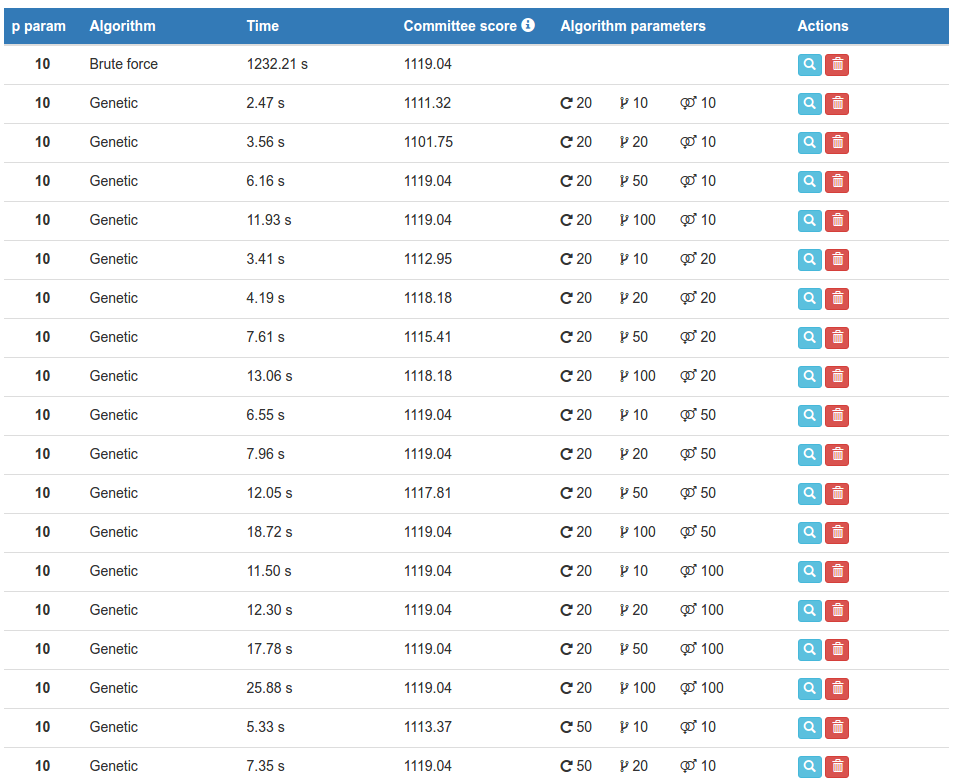
\includegraphics[width=\textwidth]{pics/porownanie-gen-brut.png}
\captionof{figure}{Porównanie wyniku algorytmu brute-force i różnych wersji algorytmu genetycznego}


\subsection{Porównanie z algorytmem zachłannym}
Dla danych z poprzedniego rozdziału algorytm zachłanny działał najszybciej, bo podał wynik już w $2,5s$, jednak o niższym wyniku, bo jedynie $1113,37$ punktów. W komitecie wskazanym przez algorytm zachłanny $2$ z $5$ kandydatów różniło się od rozwiązania najlepszego:

\begin{center}
\centerline{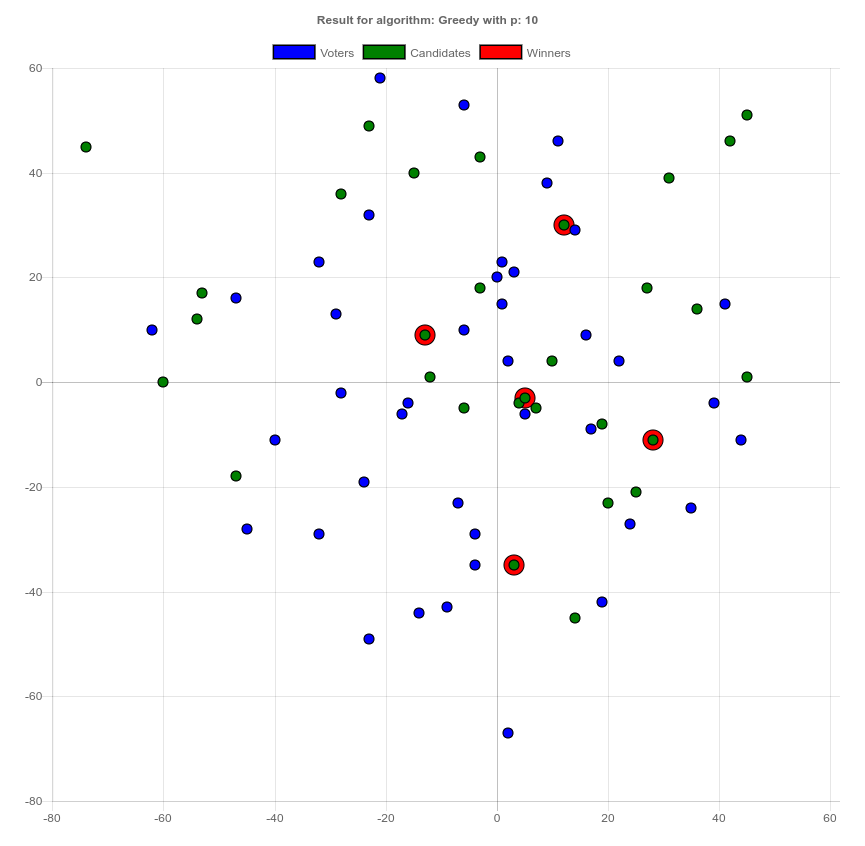
\includegraphics[width=0.6\textwidth]{pics/gg-gr.png}}
\captionof{figure}{Wynik wskazany przez algorytm zachłanny}
\end{center}
\begin{center}
\centerline{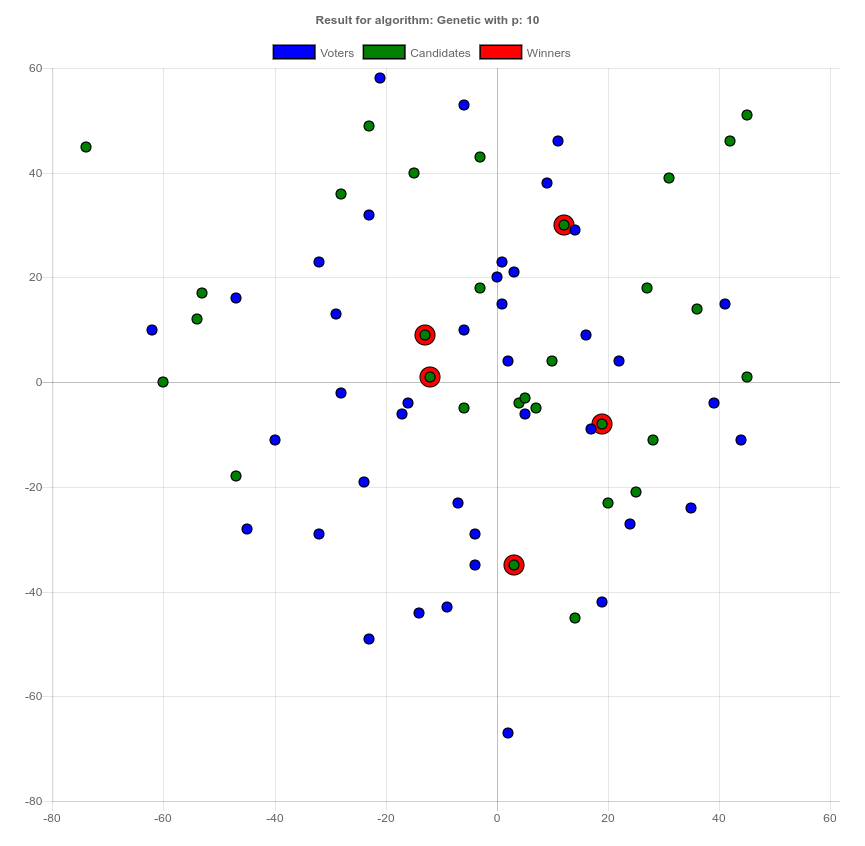
\includegraphics[width=0.6\textwidth]{pics/gg-gen.png}}
\captionof{figure}{Wynik wzorcowy wskazany przez algorytm brute-force i większość genetycznych}
\end{center}

\vspace*{-2cm}
\section{Porównanie algorytmu genetycznego z zachłannym dla różnych wartości parametru p}

Porównano wyniki i czasy działania algorytmu zachłannego zależnego od parametru $p$ i algorytmu genetycznego. Sprawdzono różne parametry działania algorytmu genetycznego. Testy przeprowadzono dla wyborów zawierających $30$ kandydatów, $50$ wyborców oraz rozmiaru komitetu liczącego $15$ zwycięzców. Sprawdzone wartości parametru $p$, to $1$, $5$ oraz $50$. Wyniki przedstawiono w postaci tabel. Zmienne znajdujące się w tabeli przy określaniu parametrów algorytmu genetycznego oznaczają odpowiednio: $c$ - liczba cykli, $m$ - prawdopodobieństwo mutacji i $k$ - zakres krzyżowania. W pierwszej tabeli przedstawiono zadowolenia wyborców z komitetów wybranych przez poszczególne algorytmy dla różnych wartości parametru $p$. W drugiej tabeli zestawiono czasy działania tychże algorytmów w sekundach.\\

\begin{center}

\begin{tabular}{|l|c|c|c|}
\hline 
parametr p & 1 & 5 & 50 \\ 
\hline 
algorytm zachłanny & 14364 & 1906.82 & 1441.4 \\ 
\hline 
algorytm genetyczny ($c=20, m=50, k=10$) & 13826 & 1889.63 & 1442.74 \\ 
\hline 
algorytm genetyczny ($c=20, m=50, k=50$) & 14274 & 1906.26 & 1446.02 \\ 
\hline 
algorytm genetyczny ($c=20, m=50, k=100$) & 14360 & 1906.82 & 1445.92 \\ 
\hline 
algorytm genetyczny ($c=20, m=100, k=10$) & 13893 & 1901.62 & 1445.92 \\ 
\hline 
algorytm genetyczny ($c=20, m=100, k=50$) & 14270 & 1906.82 & 1445.92 \\ 
\hline 
algorytm genetyczny ($c=20, m=100, k=100$) & 14364 & 1906.28 & 1446.44 \\ 
\hline 
algorytm genetyczny ($c=50, m=50, k=50$) & 14364 & 1906.82 & 1446.44 \\ 
\hline 
algorytm genetyczny ($c=50, m=100, k=100$) & 14364 & 1906.82 & 1446,44 \\ 
\hline 
\end{tabular}
\captionof{table}{Wyniki komitetów wskazanych przez poszczególne algorytmy}
\end{center} 

\begin{center}

\begin{tabular}{|l|c|c|c|}
\hline 
parametr p & 1 & 5 & 50 \\ 
\hline 
algorytm zachłanny & 2.1 & 10.87 & 11.64 \\ 
\hline 
algorytm genetyczny ($c=20, m=50, k=10$) & 3.11 & 11.14 & 13.27 \\ 
\hline 
algorytm genetyczny ($c=20, m=50, k=50$) & 4.82 & 16.15 & 18.35 \\ 
\hline 
algorytm genetyczny ($c=20, m=50, k=100$) & 6.58 & 30.21 & 26.81 \\ 
\hline 
algorytm genetyczny ($c=20, m=100, k=10$) & 5.75 & 20.83 & 23.8 \\ 
\hline 
algorytm genetyczny ($c=20, m=100, k=50$) & 8.81 & 27.65 & 29.92 \\ 
\hline 
algorytm genetyczny ($c=20, m=100, k=100$) & 10.22 & 38.44 & 44.31 \\ 
\hline 
algorytm genetyczny ($c=50, m=50, k=50$) & 11.13 & 42.85 & 45.64 \\ 
\hline 
algorytm genetyczny ($c=50, m=100, k=100$) & 24.45 & 96.06 & 103.89 \\ 
\hline 
\end{tabular}
\captionof{table}{Czasy działania algorytmów}
\end{center} 

\newpage
W poniższych tabelach zestawiono rezultaty osiągnięte przez algorytm zachłanny oraz rezultaty osiągnięte przez reprezentantów algorytmu genetycznego dla różnych parametrów $p$. Oddzielnie wybierany był reprezentant algorytmu genetycznego pod kątem jakości wyniku i czasu działania. Jeśli chodzi o reprezentanta algorytmu genetycznego pod kątem jakości wyniku, to dla każdej wartości parametru $p$ wybierano najwyższe zadowolenie wyborców osiągnięte przez algorytm genetyczny działający według jednego ze sprawdzanych zestawów parametrów działania algorytmu genetycznego. Jeśli zaś chodzi o reprezentanta algorytmu genetycznego pod kątem czasu działania, to dla danej wartości parametru $p$, wybierano najszybszy czas spośród tych wyników działania algorytmu genetycznego, które osiągnęły wartość komitetu co najmniej tak samo dobrą jak wartość komitetu uzyskana przez algorytm zachłanny dla danej wartości parametru $p$. \\

\begin{center}

\begin{tabular}{|l|c|c|}
\hline 
parametr p & algorytm zachłanny & algorytm genetyczny \\ 
\hline 
1 & 14364 & 14364 \\ 
\hline 
5 & 1906.82 & 1906.82 \\ 
\hline 
50 & 1441.4 & 1446.44 \\ 
\hline 
\end{tabular} 
\captionof{table}{Zestawienie wartości komitetów}
\end{center}

\begin{center}
\begin{tabular}{|l|c|c|}
\hline 
parametr p & algorytm zachłanny & algorytm genetyczny \\ 
\hline 
1 & 2.1 & 10.22 \\ 
\hline 
5 & 10.87 & 27.65 \\ 
\hline 
50 & 11.64 & 13.27 \\ 
\hline 
\end{tabular} 
\captionof{table}{Zestawienie czasów działania}
\end{center}

Dla każdej wartości parametru $p$ algorytm genetyczny dla pewnego zestawu parametrów działania osiągał wynik co najmniej tak samo dobry jak algorytm zachłanny. Jednocześnie czas trwania algorytmu genetycznego dla każdego przypadku był dłuższy od czasu trwania algorytmu zachłannego. Wraz ze wzrostem parametru $p$ algorytm genetyczny rósł w siłę w porównaniu z algorytmem zachłannym. Dla $p=1$ trzy z ośmiu wyników algorytmu genetycznego były tak samo dobre jak wynik algorytmu zachłannego. Dla $p=5$ już cztery z ośmiu wyników algorytmu genetycznego były tak samo dobre jak wynik algorytmu zachłannego. Z kolei dla $p=50$ każdy z wyników algorytmu genetycznego wśród badanych parametrów działania okazał się lepszy od wyniku algorytmu zachłannego. Jeśli chodzi o czas działania, to dla małych wartości parametru $p$, algorytm zachłanny wyraźnie przewyższa algorytm genetyczny. Najlepsze z wyników algorytmu genetycznego, które były co najmniej tak samo dobre jak wynik algorytmu zachłannego, obliczane były znacznie dłużej od wyniku algorytmu zachłannego. Wraz ze wzrostem parametru $p$ coraz więcej wyników algorytmu genetycznego dla różnych zestawów parametrów działania zrównuje się lub przewyższa wynik algorytmu zachłannego. W związku z tym najkrótsze czasy działania algorytmu genetycznego są coraz bliższe czasu działania algorytmu zachłannego. Dla $p=50$ czas trwania reprezentanta algorytmu genetycznego był porównywalny z czasem działania algorytmu zachłannego.  

\newpage
\cleardoublepage
\addcontentsline{toc}{chapter}{\listfigurename}
\listoffigures

\bibliographystyle{alpha}
\bibliography{bibliografia}

\end{document}
